% Options for packages loaded elsewhere
\PassOptionsToPackage{unicode}{hyperref}
\PassOptionsToPackage{hyphens}{url}
%
\documentclass[
]{book}
\usepackage{amsmath,amssymb}
\usepackage{lmodern}
\usepackage{ifxetex,ifluatex}
\ifnum 0\ifxetex 1\fi\ifluatex 1\fi=0 % if pdftex
  \usepackage[T1]{fontenc}
  \usepackage[utf8]{inputenc}
  \usepackage{textcomp} % provide euro and other symbols
\else % if luatex or xetex
  \usepackage{unicode-math}
  \defaultfontfeatures{Scale=MatchLowercase}
  \defaultfontfeatures[\rmfamily]{Ligatures=TeX,Scale=1}
\fi
% Use upquote if available, for straight quotes in verbatim environments
\IfFileExists{upquote.sty}{\usepackage{upquote}}{}
\IfFileExists{microtype.sty}{% use microtype if available
  \usepackage[]{microtype}
  \UseMicrotypeSet[protrusion]{basicmath} % disable protrusion for tt fonts
}{}
\makeatletter
\@ifundefined{KOMAClassName}{% if non-KOMA class
  \IfFileExists{parskip.sty}{%
    \usepackage{parskip}
  }{% else
    \setlength{\parindent}{0pt}
    \setlength{\parskip}{6pt plus 2pt minus 1pt}}
}{% if KOMA class
  \KOMAoptions{parskip=half}}
\makeatother
\usepackage{xcolor}
\IfFileExists{xurl.sty}{\usepackage{xurl}}{} % add URL line breaks if available
\IfFileExists{bookmark.sty}{\usepackage{bookmark}}{\usepackage{hyperref}}
\hypersetup{
  pdftitle={Boosting methods: Theory and application in R},
  pdfauthor={Emanuel Sommer},
  hidelinks,
  pdfcreator={LaTeX via pandoc}}
\urlstyle{same} % disable monospaced font for URLs
\usepackage{color}
\usepackage{fancyvrb}
\newcommand{\VerbBar}{|}
\newcommand{\VERB}{\Verb[commandchars=\\\{\}]}
\DefineVerbatimEnvironment{Highlighting}{Verbatim}{commandchars=\\\{\}}
% Add ',fontsize=\small' for more characters per line
\usepackage{framed}
\definecolor{shadecolor}{RGB}{248,248,248}
\newenvironment{Shaded}{\begin{snugshade}}{\end{snugshade}}
\newcommand{\AlertTok}[1]{\textcolor[rgb]{0.94,0.16,0.16}{#1}}
\newcommand{\AnnotationTok}[1]{\textcolor[rgb]{0.56,0.35,0.01}{\textbf{\textit{#1}}}}
\newcommand{\AttributeTok}[1]{\textcolor[rgb]{0.77,0.63,0.00}{#1}}
\newcommand{\BaseNTok}[1]{\textcolor[rgb]{0.00,0.00,0.81}{#1}}
\newcommand{\BuiltInTok}[1]{#1}
\newcommand{\CharTok}[1]{\textcolor[rgb]{0.31,0.60,0.02}{#1}}
\newcommand{\CommentTok}[1]{\textcolor[rgb]{0.56,0.35,0.01}{\textit{#1}}}
\newcommand{\CommentVarTok}[1]{\textcolor[rgb]{0.56,0.35,0.01}{\textbf{\textit{#1}}}}
\newcommand{\ConstantTok}[1]{\textcolor[rgb]{0.00,0.00,0.00}{#1}}
\newcommand{\ControlFlowTok}[1]{\textcolor[rgb]{0.13,0.29,0.53}{\textbf{#1}}}
\newcommand{\DataTypeTok}[1]{\textcolor[rgb]{0.13,0.29,0.53}{#1}}
\newcommand{\DecValTok}[1]{\textcolor[rgb]{0.00,0.00,0.81}{#1}}
\newcommand{\DocumentationTok}[1]{\textcolor[rgb]{0.56,0.35,0.01}{\textbf{\textit{#1}}}}
\newcommand{\ErrorTok}[1]{\textcolor[rgb]{0.64,0.00,0.00}{\textbf{#1}}}
\newcommand{\ExtensionTok}[1]{#1}
\newcommand{\FloatTok}[1]{\textcolor[rgb]{0.00,0.00,0.81}{#1}}
\newcommand{\FunctionTok}[1]{\textcolor[rgb]{0.00,0.00,0.00}{#1}}
\newcommand{\ImportTok}[1]{#1}
\newcommand{\InformationTok}[1]{\textcolor[rgb]{0.56,0.35,0.01}{\textbf{\textit{#1}}}}
\newcommand{\KeywordTok}[1]{\textcolor[rgb]{0.13,0.29,0.53}{\textbf{#1}}}
\newcommand{\NormalTok}[1]{#1}
\newcommand{\OperatorTok}[1]{\textcolor[rgb]{0.81,0.36,0.00}{\textbf{#1}}}
\newcommand{\OtherTok}[1]{\textcolor[rgb]{0.56,0.35,0.01}{#1}}
\newcommand{\PreprocessorTok}[1]{\textcolor[rgb]{0.56,0.35,0.01}{\textit{#1}}}
\newcommand{\RegionMarkerTok}[1]{#1}
\newcommand{\SpecialCharTok}[1]{\textcolor[rgb]{0.00,0.00,0.00}{#1}}
\newcommand{\SpecialStringTok}[1]{\textcolor[rgb]{0.31,0.60,0.02}{#1}}
\newcommand{\StringTok}[1]{\textcolor[rgb]{0.31,0.60,0.02}{#1}}
\newcommand{\VariableTok}[1]{\textcolor[rgb]{0.00,0.00,0.00}{#1}}
\newcommand{\VerbatimStringTok}[1]{\textcolor[rgb]{0.31,0.60,0.02}{#1}}
\newcommand{\WarningTok}[1]{\textcolor[rgb]{0.56,0.35,0.01}{\textbf{\textit{#1}}}}
\usepackage{longtable,booktabs,array}
\usepackage{calc} % for calculating minipage widths
% Correct order of tables after \paragraph or \subparagraph
\usepackage{etoolbox}
\makeatletter
\patchcmd\longtable{\par}{\if@noskipsec\mbox{}\fi\par}{}{}
\makeatother
% Allow footnotes in longtable head/foot
\IfFileExists{footnotehyper.sty}{\usepackage{footnotehyper}}{\usepackage{footnote}}
\makesavenoteenv{longtable}
\usepackage{graphicx}
\makeatletter
\def\maxwidth{\ifdim\Gin@nat@width>\linewidth\linewidth\else\Gin@nat@width\fi}
\def\maxheight{\ifdim\Gin@nat@height>\textheight\textheight\else\Gin@nat@height\fi}
\makeatother
% Scale images if necessary, so that they will not overflow the page
% margins by default, and it is still possible to overwrite the defaults
% using explicit options in \includegraphics[width, height, ...]{}
\setkeys{Gin}{width=\maxwidth,height=\maxheight,keepaspectratio}
% Set default figure placement to htbp
\makeatletter
\def\fps@figure{htbp}
\makeatother
\setlength{\emergencystretch}{3em} % prevent overfull lines
\providecommand{\tightlist}{%
  \setlength{\itemsep}{0pt}\setlength{\parskip}{0pt}}
\setcounter{secnumdepth}{5}
\usepackage{booktabs}
\usepackage{array}
\ifluatex
  \usepackage{selnolig}  % disable illegal ligatures
\fi
\usepackage[]{natbib}
\bibliographystyle{apalike}
\newlength{\cslhangindent}
\setlength{\cslhangindent}{1.5em}
\newlength{\csllabelwidth}
\setlength{\csllabelwidth}{3em}
\newenvironment{CSLReferences}[2] % #1 hanging-ident, #2 entry spacing
 {% don't indent paragraphs
  \setlength{\parindent}{0pt}
  % turn on hanging indent if param 1 is 1
  \ifodd #1 \everypar{\setlength{\hangindent}{\cslhangindent}}\ignorespaces\fi
  % set entry spacing
  \ifnum #2 > 0
  \setlength{\parskip}{#2\baselineskip}
  \fi
 }%
 {}
\usepackage{calc}
\newcommand{\CSLBlock}[1]{#1\hfill\break}
\newcommand{\CSLLeftMargin}[1]{\parbox[t]{\csllabelwidth}{#1}}
\newcommand{\CSLRightInline}[1]{\parbox[t]{\linewidth - \csllabelwidth}{#1}\break}
\newcommand{\CSLIndent}[1]{\hspace{\cslhangindent}#1}

\title{Boosting methods: Theory and application in R}
\author{Emanuel Sommer}
\date{2021-06-18}

\begin{document}
\maketitle

{
\setcounter{tocdepth}{1}
\tableofcontents
}
\hypertarget{prerequisites}{%
\chapter{Prerequisites}\label{prerequisites}}

The reader should have some basic knowledge of the following topics:

\begin{itemize}
\item
  Statistical learning

  \begin{itemize}
  \item
    Train/ test split
  \item
    Cross-validation
  \item
    Overfitting
  \item
    Gradient descent
  \item
    Bias variance trade-off
  \item
    Hyperparameters
  \end{itemize}
\item
  Regression trees and random forest models
\item
  Basic R knowledge (only for the applied part)
\end{itemize}

\hypertarget{intro}{%
\chapter{Introduction}\label{intro}}

This bookdown project shows my work for the main master's seminar from my \emph{M.Sc. Mathematics in Data Science} at the TUM. The topic of the seminar is \emph{Statistical Methods and Models}. During the seminar I was supervised by Prof.~Claudia Czado and Özge Sahin. My topic and thus covered in this project are boosting methods. Those are unarguably one of the hottest machine learning algorithms for tabular data to date.

\begin{quote}
``Boosting is one of the most powerful learning ideas introduced in the last
twenty years.'' \citep{elements}
\end{quote}

Hereby the focus will lie on the regression and not the more often discussed classification setting. The main idea of boosting is to sequentially build models from some class of base learners to finally combine them to a powerful ensemble model. As the base learners regression trees will be chosen in this project.

The next chapter will cover the theory behind boosting and especially tree-based gradient boosting. Besides a very prominent, efficient and successful implementation of tree-based gradient boosting namely XGBoost will be discussed in this chapter. It gained a lot of attention when it was integral to many winning submissions in machine learning competitions on the platform Kaggle and comes with some interesting tweaks to the general algorithm.

The application of the discussed boosting models to two real world data sets with the use of the programming language R are the content of the subsequent chapters. This will be divided into exploratory data analysis and the modeling itself. Notably the framework of \texttt{tidymodels} is used in the practical part.

\hypertarget{theory}{%
\chapter{Theory}\label{theory}}

\hypertarget{the-powerful-idea-of-gradient-boosting}{%
\section{The powerful idea of gradient boosting}\label{the-powerful-idea-of-gradient-boosting}}

As roughly mentioned in the introduction section \ref{intro} the main idea of boosting is to sequentially build weak learners that form a powerful ensemble model. With weak learners models with high bias and low variance are meant that perform at least a little better than guessing. This already shows that the sequential approach of gradient boosting with weak learners stands in strong contrast to bagged ensembles like random forest. There many models with low bias and high variance are fitted in a parallel fashion and the variance is then reduced by averaging over the models.\citep{HandsOnMLwithR} It is not totally clear from which field boosting methods emerged but some claim that the work of Freund and Schapire with respect to PAC learning in the 1990s were instrumental for their growth.\citep{elements} PAC learning can be considered one field within the broader field of learning theory that tries to find generalization bounds for algorithms that are probably approximately correct (PAC).\citep{pacbounds} This section will first cover the general setup of gradient boosting as the most prominent method to train forward stagewise additive models. Secondly tree-based gradient boosting and finally a very efficient and robust tree-based gradient boosting algorithm namely XGBoost will be discussed in detail.

\hypertarget{forward-stagewise-additive-modeling}{%
\subsection{Forward Stagewise Additive Modeling}\label{forward-stagewise-additive-modeling}}

In the setting of the data set \(\mathcal{D} = \{(y_i,x_i)\ | i \in [N]\}\) with predictors \(x_i \in \mathbb{R}^m\) and target \(y_i \in \mathbb{R}\) boosting is fitting the following additive, still quite general, model.

\begin{equation}
  \hat{y_i} = \phi(x_i) = \sum_{k=1}^{K} f_k(x_i), \quad f_k \in \mathcal{F}
  \label{eq:additiveModel}
\end{equation}

Where \(\mathcal{F}\) is the space of learning algorithms that will be narrowed down later on. Additive expansions like this are at the core of many other powerful machine learning algorithms like Neural Networks or Wavelets.\citep{elements}

The formulation \eqref{eq:additiveModel} leads to so called forward stagewise additive modeling which basically means that one sequentially adds \(f \in \mathcal{F}\) to the current model \(\phi_k\) without changing anything about the previous models.\citep{elements} The algorithm is shown below.

\begin{center}\rule{0.5\linewidth}{0.5pt}\end{center}

\textbf{Algorithm 1}: Forward Stagewise Additive Modeling \citep{elements}

\begin{center}\rule{0.5\linewidth}{0.5pt}\end{center}

\begin{enumerate}
\def\labelenumi{\arabic{enumi}.}
\item
  Initialize \(\phi_0(x) = 0\)
\item
  For \(k = 1\) to \(K\) do:

  \begin{itemize}
  \tightlist
  \item
    \((\beta_k,\gamma_k) = argmin_{\beta,\gamma}\sum_{i=1}^N L(y_i,\phi_{k-1}(x_i) + \beta f(x_i,\gamma))\)
  \item
    \(\phi_k(x) = \phi_{k-1}(x) + \beta_k f(x, \gamma_k)\)
  \end{itemize}
\end{enumerate}

Where \(\gamma\) parameterizes the learner \(f \in \mathcal{F}\) and the \(\beta_k\) are the expansion coefficients. \(L\) should be a differentiable loss function.

\begin{center}\rule{0.5\linewidth}{0.5pt}\end{center}

For example for the basic \(L_2\) loss the expression to be minimized simplifies to the following:

\[
L_2(y_i,\phi_{k-1}(x_i) + \beta f(x_i,\gamma)) = (y_i - \phi_{k-1}(x_i) - \beta f(x_i,\gamma))^2
\]

As \(y_i - \phi_{k-1}(x_i)\) is just the residual of the previous model, the next model that is added corresponds to the model that best approximates the residuals of the current model. Although the \(L_2\) loss has many very nice properties like the above, it lacks robustness against outliers. Therefore two alternative losses for boosting in the regression setting are worth considering.

\hypertarget{robust-loss-functions-for-regression}{%
\subsection{Robust loss functions for regression}\label{robust-loss-functions-for-regression}}

As the \(L_2\) loss squares the residuals, observations with large absolute residuals are overly important in the minimization step. This effect can be reduced intuitively by just using the \(L_1\) loss i.e.~minimize over the sum over just the absolute residuals. To do this is indeed a valid approach and can reduce the influence of outliers greatly and thus make the final model more robust. Another good choice could be the \textbf{Huber} loss which tries to get the best of \(L_1\) and \(L_2\) loss.\citep{elements}

\begin{equation}
  L_{Huber}(y,f(x)) = \begin{cases}L_2(y,f(x)) & |y-f(x)| \leq \delta \\
  2\delta |y-f(x)| - \delta^2 & otherwise.
  \end{cases}
  \label{eq:huberLoss}
\end{equation}

In Figure \ref{fig:lossComp} is a comparison of the three different losses discussed so far.\citep{elements}

\begin{figure}

{\centering \includegraphics[width=0.7\linewidth]{_pictures/huber_loss} 

}

\caption{Comparison of different regression loss functions.}\label{fig:lossComp}
\end{figure}

These alternative loss criteria are more robust but make the fitting i.e.~the minimization much more complex as they do not yield such simplifications like the \(L_2\) loss.\citep{elements} The next step in the journey of exploring boosting is to narrow down the argument spaces of \textbf{Algorithm 1} (Forward Stagewise Additive Modeling) and to specify a subset of the general space of learning algorithms. This subset will be the space of Classification and Regression Tree (CART) models and in this case as the focus is on a regression task the space of regression trees. This choice is by no means arbitrary as in practice tree-based boosting algorithms have proven countless of times that they provide very robust and accurate models but still other learners might be chosen.\citep[\citet{HandsOnMLwithR}]{elements} The next subsection will explore how one can actually fit such a forward stagewise additive model when using regression trees as the learner class.

\hypertarget{general-gradient-tree-boosting}{%
\section{General gradient tree boosting}\label{general-gradient-tree-boosting}}

From now on there is the switch from the space of learning algorithms \(\mathcal{F}\) to the space of regression trees \(\mathcal{T}\). Such a regression tree can be formally expressed by:

\begin{equation}
  t(x, \gamma, R) = \sum_{j=1}^J \gamma_j I(x \in R_j) \quad \text{for  } t \in \mathcal{T}
  \label{eq:treeDef}
\end{equation}

With \(R_j\) being \(J\) distinct regions of the predictor space usually attained by recursive binary splitting. Moreover these regions correspond to the leafs of the tree and the number of leafs \(J\) or the depth of the trees are most often hyperparameters (not trained). The \(\gamma_j \in \mathbb{R}\) are the predictions for a given x if x is contained in the region \(R_j\). While it is quite easy to get the \(\gamma_j\) for the regions given, most often by computing \(\gamma_j = \frac{1}{|\{x \in R_j\}|} \sum_{\{x \in R_j\}} x\) , it is a much harder problem to get good distinct regions. The above mentioned recursive binary splitting is an approximation to do this and works in a top down greedy fashion.\citep{elements} From now on we assume that we have an efficient way of fitting such trees to a metric outcome variable e.g.~by recursive binary splitting.

A nice graphical example of an additive model based on trees is displayed in the figure \ref{fig:exampleAdditiveTree} below.\citep{xgboostPaper}

\begin{figure}

{\centering \includegraphics[width=0.7\linewidth]{_pictures/boosting_easy} 

}

\caption{Example of an additive tree ensamble.}\label{fig:exampleAdditiveTree}
\end{figure}

Having now the new space \(\mathcal{T}\) for the general boosting model \eqref{eq:additiveModel} one can write down the optimization problem that has to be solved in each step of the forward stagewise process of fitting the model.

\begin{equation}
  (\gamma^{(k)},R^{(k)}) = argmin_{\gamma,R} \sum_{i=1}^N L(y_i, \phi_{k-1}(x_i) + t(x_i,\gamma,R))
  \label{eq:oneStepTreeBoost}
\end{equation}

This can be estimated fast and quite straight forward if there is a simplification like the one seen for the \(L_2\) loss. But in the more general case of an arbitrary differentiable convex loss function like the Huber loss techniques from numerical optimization are needed to derive fast algorithms.\citep{elements}

\hypertarget{numOpt}{%
\subsection{Numerical optimization}\label{numOpt}}

According to \textbf{Algorithm 1} the goal in order to fit the boosting model is to minimize over the full loss of the training data \(\mathcal{D}\) which is the sum over all observation losses.

\[
L(\phi) = \sum_{i=1}^N L(y_i, \phi(x_i))
\]

And thus the \(\hat{\phi}\) additive boosting model we try to get is the following.

\[
\hat{\phi} = argmin_{\phi} L(\phi)
\]

Now we basically follow the spirit of the general gradient descent algorithm for differentiable functions. In the general case we minimize a function \(f(x)\) by stepping iteratively along the direction of the steepest descent i.e.~the negative gradient. The step length can then either be a constant small scalar or be determined by a line search.

In the setting of the additive boosting model \(\phi\) can be viewed as a vector of dimension \(N\) that contains the prediction according to \(\phi\) of the corresponding observation i.e.~\(\phi = (\phi(x_1),...,\phi(x_N))\). So the loss function \(L(\phi)\) corresponds to the \(f(x)\) in the general gradient descent algorithm. Numerical optimization, here gradient descent, then solves for \(\hat{\phi}\) by a sum of vectors of the same dimension as the \(\phi\).\citep{elements} The result of the sum \(\phi_K\) (\eqref{eq:numOptSol}) can be viewed as the current proposal for the optimal \(\hat{\phi}\) after \(K\) optimization steps and each \(h^{(k)}\) is the proposed improvement step.

\begin{equation}
  \phi_K = \sum_{k=0}^K h^{(k)} \quad h^{(k)} \in \mathbb{R}^N 
  \label{eq:numOptSol}
\end{equation}

While \(h^{(0)}\) is just an initial guess the subsequent \(h^{(k)}\) are again the prediction vectors of the corresponding model out of \(\mathcal{T}\) i.e.~\(h^{(k)}_{i} = t_k(x_i)\) with \(t \in \mathcal{T}\). This means that each \(\phi_k = \phi_{k-1} + h^{(k)}\). The \(h^{(k)}\) are calculated via the gradient which finally comes into play. As mentioned above one minimizes the loss the most by going towards the direction of the steepest descent. For \eqref{eq:numOptSol} follows from its additive formulation and defining \(g^{(k)}\) as the gradient of \(L(\phi_k)\) evaluated for \(\phi_{k-1}\) the update \(h^{(k)} = -\lambda_k g^{(k)}\). As we assumed the loss to be differentiable we see that \(g^{(k)}\) is well defined. Here \(\lambda_k\) is the usual step length for gradient descent methods. It is the solution of the line search \(\lambda_k = argmin_{\lambda} L(\phi_{k-1} - \lambda g^{(k)})\). This \(\lambda_k\) almost exactly corresponds to the \(\beta_k\) in \textbf{Algorithm 1} although here the optimization is performed for every region of the tree separately.\citep{elements}

With these insights it is clear that the tree predictions correspond to the negative gradient \(-g^{(k)}\). Of course the predictions are not independent as the prediction is constant for each leaf of the tree. So the new optimization proposed by numerical optimization via gradient boosting is given in \eqref{eq:oneStepTreeBoostnew} below.

\begin{equation}
  (\tilde{\gamma}^{(k)},\tilde{R}^{(k)}) = argmin_{\gamma,R} \sum_{i=1}^N [-g^{(k)}_{i} -  t(x_i,\gamma,R)] ^2
  \label{eq:oneStepTreeBoostnew}
\end{equation}

In words this just means fitting a regression tree by least squares to the negative gradients that were evaluated with the current predictions. The solution regions will not exactly match the ones from \eqref{eq:oneStepTreeBoost} but should be very similar.\citep{elements} After having estimated the regions one estimates the parameters \(\gamma\) by solving the line search \eqref{eq:gammaLineSearch}.

\begin{equation}
  \tilde{\gamma}^{(k)}_{j} = argmin_{\gamma^{(k)}_{j}} \sum_{x \in R^{(k)}_{j}} L(y_i,\phi_{k-1}(x_i) + \gamma^{(k)}_{j})
  \label{eq:gammaLineSearch}
\end{equation}

Putting all of this back together with \textbf{Algorithm 1} results in \textbf{Algorithm 2} that covers a general algorithm for tree-based gradient boosting.

\begin{center}\rule{0.5\linewidth}{0.5pt}\end{center}

\textbf{Algorithm 2}: Tree-based gradient boosting \citep{elements}

\begin{center}\rule{0.5\linewidth}{0.5pt}\end{center}

\begin{enumerate}
\def\labelenumi{\arabic{enumi}.}
\item
  Initialize \(\phi_0(x)\) as a singular node tree.
\item
  For \(k = 1\) to \(K\) do:

  \begin{itemize}
  \item
    For \(i = 1\) to \(N\) compute:

    \(g^{(k)}_{i} = \bigg[\frac{\partial L(y_i, \phi(x_i))}{\partial \phi(x_i)}\bigg]_{\phi = \phi_{k-1}}\)
  \item
    Fit a regression tree by least squares to the outcome vector \(-g^{(k)}\) in order to get the \(J^{(k)}\) distinct regions \(\tilde{R}^{(k)}_j\).
  \item
    For each of these \(J^{(k)}\) regions perform a line search in order to compute the leaf predictions \(\tilde{\gamma}^{(k)}_{j}\) exactly like in \eqref{eq:gammaLineSearch}.
  \item
    Set \(\phi_k(x) = \phi_{k-1}(x) + t(x,\tilde {\gamma}^{(k)}_{j},\tilde{R}^{(k)}_j)\) with \(t \in \mathcal{T}\)
  \end{itemize}
\end{enumerate}

\begin{center}\rule{0.5\linewidth}{0.5pt}\end{center}

The only unknowns in this algorithm are now the differentiable loss function and the hyperparameters like the \(J^{(k)}\) and the \(K\). While choices for the hyperparameters are discussed further below, the following table \ref{tab:lossGradients} displays the gradients for the losses discussed so far.

\begin{longtable}[]{@{}
  >{\raggedright\arraybackslash}p{(\columnwidth - 2\tabcolsep) * \real{0.27}}
  >{\raggedright\arraybackslash}p{(\columnwidth - 2\tabcolsep) * \real{0.73}}@{}}
\caption{\label{tab:lossGradients} Gradients of the discussed losses \citep{elements}}\tabularnewline
\toprule
Loss & Gradient \\
\midrule
\endfirsthead
\toprule
Loss & Gradient \\
\midrule
\endhead
\(L_2\): \((y_i - \phi(x_i))^2\) & \(2(y_i - \phi(x_i))\) \\
\(L_1\): \(|y_i - \phi(x_i)|\) & \(sign(y_i - \phi(x_i))\) \\
Huber loss \eqref{eq:huberLoss} & \(y_i - \phi(x_i)\) for \(|y_i - \phi(x_i)| \leq \delta\)

\(\delta sign(y_i - \phi(x_i))\) otherwise, with \(\delta\) quantile of \(|y_i - \phi(x_i)|\) \\
\bottomrule
\end{longtable}

\hypertarget{single-tree-depth}{%
\subsection{Single tree depth}\label{single-tree-depth}}

The question which \(J^{(k)}\) should be used at each iteration is now shortly discussed. Basically using the tree depth (\(log_2(J^{(k)}) = Depth^{(k)}\)) of one means allowing only the main effects and no interactions. A value of 2 already allows all two way interaction effects and so on. As one stacks these models additive and does not restrict oneself to a single one, the building of a large tree and then pruning it back at each iteration as the regular CART algorithms do would be a computational overkill. Instead it has proven to be sufficient and efficient in practice to set the values \(Depth^{(k)}\) to a constant \(Depth \approx 6\).\citep{elements} Also decision stumps (\(Depth = 1\)) could be used but may require a lot more iterations.

\hypertarget{combOver}{%
\subsection{Combat overfitting}\label{combOver}}

No learning algorithm could be fully covered without treating the good old problem of overfitting. In the setting of boosting the experienced eye could have spotted the problem of overfitting already in the definition of the additive model \eqref{eq:additiveModel}. There the number \(K\) of models that form the ensemble was introduced but was not discussed further till now. Of course one can arbitrarily fit or better say remember some given training data in order to minimize the loss with such an additive model by letting \(K\) be arbitrarily large. This comes from the fact that the loss reduces usually after each iteration over \(K\).\citep{elements} The easiest way to prevent overfitting is to have a validation set at hand which is disjoint from the training data. Having such a validation set at hand can be used to monitor the loss on the unseen data. In the case the loss would rise again on the validation data one can consider to stop the algorithm and to use the current iteration number for the final parameter \(K\). This approach is often called early stopping. Besides that there are methods that regularize the individual trees that are fitted in each iteration. Two of those will be discussed now.

\hypertarget{shrinkage}{%
\subsubsection{Shrinkage}\label{shrinkage}}

Shrinkage basically refers to just introducing a learning rate \(\eta\). This learning rate \(\eta\) scales the contribution of the new model. In general the learning rate should be in \((0,1]\) but in practice it has been shown that rather small values like \(\eta < 0.1\) work very good.\citep{elements} As almost everything in life this does not come for free. A smaller learning rate usually comes with a computational cost as with lower \(\eta\) a larger \(K\) is required. Those two hyperparameters represent a trade-off in a way. In practice it is advisable to use a small learning rate \(\eta\) and adjust the \(K\) accordingly which in this case would mean to make the \(K\) large enough until one reaches an early stopping point. Still it is good to keep in mind that a \(\eta\) that is too small can lead to an immense and unnecessary computational effort. All in all using shrinkage the update step in \textbf{Algorithm 2} changes to the following.

\begin{equation}
  \phi_k(x) = \phi_{k-1}(x) + \eta * t(x,\tilde {\gamma}^{(k)}_{j},\tilde{R}^{(k)}_j)
  \label{eq:shrinkage}
\end{equation}

\hypertarget{subsampling}{%
\subsubsection{Subsampling}\label{subsampling}}

The other method to regularize the trees will be subsampling. There are two different kinds of subsampling. The first one is row-subsampling which basically means just using a random fraction of the training data in each iteration when fitting the new tree. Common values are \(\frac{1}{2}\) but for a larger training set the value can be chosen to be smaller. This does not only help to prevent overfitting and thus achieving a better predictive performance but reduces also the computational effort in each iteration.\citep{elements} The approach is very similar to the dropout technique in the setting of deep neural networks.

Moreover one can apply column-subsampling or feature-subsampling. Here only a fraction of the features or an explicit number of the features are used in each iteration. This is the exact same method and intention as the one applied in random forest models. Again the technique not only boosts performance on unseen data but also reduces the computational time.\citep{xgboostPaper} Still it must be noted that by using one or both subsampling methods one introduces one or two additional hyperparameters to the model that have to be tuned.

Having the \textbf{Algorithm 2} for tree-based gradient boosting alongside some regularization techniques it is time to look at a very popular, efficient and powerful open source implementation.

\hypertarget{xgboost-a-highly-efficient-implementation}{%
\section{XGBoost a highly efficient implementation}\label{xgboost-a-highly-efficient-implementation}}

The XGBoost algorithm is a highly scalable, efficient and successful implementation and optimization of \textbf{Algorithm 2} introduced by Chen and Guestrin in 2016.\citep[\citet{HandsOnMLwithR}]{xgboostPaper} It has gained a lot of spotlight when it was integral for many winning submissions at kaggle machine learning challenges. In the following the most important tweaks that are proposed to \textbf{Algorithm 2} are covered.

\hypertarget{regularized-loss}{%
\subsection{Regularized loss}\label{regularized-loss}}

Instead of just minimizing a convex and differentiable loss \(L\) XGBoost minimizes the following regularized loss.\citep{xgboostPaper}

\begin{equation}
  \begin{split}
  \mathcal{L}(\phi) = L(\phi) + \sum_{k=1}^K \Omega(t_k) \\
  \text{where } \Omega(t) = \nu J + \frac{1}{2} \lambda ||\gamma||^2 \quad t \in \mathcal{T}
  \end{split}
  \label{eq:regLoss}
\end{equation}

Here \(J\) and \(\gamma\) again parameterize the regression trees \(t \in \mathcal{T}\) as defined in \eqref{eq:treeDef}. As evident from the formula both hyperparameters \(\nu\) and \(\lambda\) favor when increased less complex models at each iteration. This is again a measure against overfitting.

This regularized objective leads to a slightly modified version of the minimization problem \eqref{eq:oneStepTreeBoost} that has to be solved in each iteration.

\begin{equation}
  (\gamma^{(k)},R^{(k)}) = argmin_{\gamma,R} \sum_{i=1}^N L(y_i, \phi_{k-1}(x_i) + t(x_i,\gamma,R)) + \Omega(t(x_i,\gamma,R))
  \label{eq:oneStepXGBoost}
\end{equation}

Instead of the first order approach, that has been introduced in \ref{numOpt}, XGBoost uses a second order approximation to further simplify the objective. This means that besides the first order gradient \(g^{(k)}\) of the loss function evaluated at \(\phi_{k-1}\) also the second order gradient \(z^{(k)}_i = \bigg[\frac{\partial^2 L(y_i, \phi(x_i))}{\partial^2 \phi(x_i)}\bigg]_{\phi = \phi_{k-1}}\) is used. By neglecting constants one reaches the approximate new objective below.\citep{xgboostPaper}

\begin{equation}
\begin{split}
  \tilde{\mathcal{L}}^{(k)} & = \sum_{i=1}^N [g^{(k)}_i t^{(k)}(x_i) + \frac{1}{2} t^{(k)}(x_i)^2] + \Omega(t^{(k)}) \\
  & = \sum_{j=1}^J [(\sum_{\{i|x_i \in R^{(k)}_j\}} g^{(k)}_i) \gamma^{(k)}_j + \frac{1}{2} (\sum_{\{i|x_i \in R^{(k)}_j\}} z^{(k)}_i + \lambda) (\gamma^{(k)}_j)^2 ] + \nu J
\end{split}
\label{eq:oneappStepXGBoost}
\end{equation}

This representation is used as it can be decomposed by the \(J\) leafs of the tree. One can then define a scoring function for split finding that only depends on \(g^{(k)}\) and \(z^{(k)}\). This approach speeds up the split finding and allows further parallel computations with respect to the leafs.

\hypertarget{shrinkage-and-subsampling}{%
\subsection{Shrinkage and subsampling}\label{shrinkage-and-subsampling}}

As discussed above in \ref{combOver} shrinkage and subsampling are great ways to regularize the model and prevent overfitting. XGBoost implements both shrinkage and subsampling. It enables the user to use column as well as row subsampling. The authors claim that in practice column subsampling has prevented overfitting more than row subsampling.\citep{xgboostPaper}

\hypertarget{even-more-tweaks}{%
\subsection{Even more tweaks}\label{even-more-tweaks}}

Besides the changes above the authors also implemented an effective approximate algorithm for split finding for the tree building step. A very nice attribute of this approximate procedure is that the algorithm is sparsity aware i.e.~the processing of missing values or 0 values is very efficient. This is done via a learned default direction in each split. Moreover they used very efficient data structures to allow a lot of parallel processing.\citep{xgboostPaper} It is written in C++ but has APIs in various languages like in R via the \texttt{xgboost} package.\citep{xgboost_package}

\hypertarget{hyperparameters-overview}{%
\subsection{Hyperparameters overview}\label{hyperparameters-overview}}

As the \textbf{tidymodels} framework will be used in the applied part, the according names from the parsnip interface for tree-based boosting i.e.~\texttt{boost\_tree} are shown below.\citep[\citet{xgboost_package}, \citet{tidymodels}]{xgboostPaper}

\begin{longtable}[]{@{}
  >{\raggedright\arraybackslash}p{(\columnwidth - 4\tabcolsep) * \real{0.14}}
  >{\raggedright\arraybackslash}p{(\columnwidth - 4\tabcolsep) * \real{0.16}}
  >{\raggedright\arraybackslash}p{(\columnwidth - 4\tabcolsep) * \real{0.70}}@{}}
\caption{\label{tab:xgboostHyper} XGBoost hyperparameters overview.}\tabularnewline
\toprule
Hyperparameter & Notation above & Meaning \\
\midrule
\endfirsthead
\toprule
Hyperparameter & Notation above & Meaning \\
\midrule
\endhead
\texttt{trees} & \(K\) & Number of trees in the ensemble. \\
\texttt{tree\_depth} & \(max(log_2J^{(k)})\) & Maximum depth of the trees. \\
\texttt{learn\_rate} & \(\eta\) & Learning rate (shrinkage). \\
\texttt{min\_n} & & Minimum number of observations in terminal region \(R^{(k)}_j\). \\
\texttt{lambda} & \(\lambda\) & \(L_2\) regularization parameter on \(\gamma\) as in \eqref{eq:oneappStepXGBoost} (default = 0). \\
\texttt{alpha} & & \(L_1\) regularization parameter on \(\gamma\) (default = 0). \\
\texttt{loss\_reduction} & \(\nu\) & Minimal loss reduction for terminal partitions. (default = 0) \\
\texttt{mtry} & & Proportion or number of columns for column subsampling. \\
\texttt{sample\_size} & & Proportion of observations for row subsampling. \\
\texttt{stop\_iter} & & Allowed number of rounds without improvement before early stopping. \\
\bottomrule
\end{longtable}

Note that the \(L_1\) penalization term would be added to the \(\Omega\) term in the loss \(\mathcal{L}\) of XGBoost.

This closes the chapter on the theory of boosting methods with a focus on tree-based gradient boosting. The discussed tools will be put to the test in the subsequent sections where real world data will be analyzed with them.

\hypertarget{eda}{%
\chapter{Explore the data}\label{eda}}

Before one starts with the actual modeling it is crucial to get to know the data and to bring it to the correct format. This process of getting familiar with the data is well known as Exploratory Data Analysis (EDA). To do this many packages are used.\citetext{\citealp{tidyverse}; \citealp{tidymodels}; \citealp{viridis}; \citealp{ggtext}; \citealp[ ]{viridisLite}; \citealp{patchwork}; \citealp{visdat}; \citealp{lubridate}; \citealp{latexplots}; \citealp{ggally}} The most important ones will be loaded below.

\begin{Shaded}
\begin{Highlighting}[]
\FunctionTok{library}\NormalTok{(tidyverse) }\CommentTok{\# general data handling tools}
\FunctionTok{library}\NormalTok{(tidymodels) }\CommentTok{\# data modeling and preprocessing}
\CommentTok{\# color palettes}
\FunctionTok{library}\NormalTok{(viridis)}
\FunctionTok{library}\NormalTok{(viridisLite)}
\FunctionTok{library}\NormalTok{(patchwork) }\CommentTok{\# composing of ggplots}
\end{Highlighting}
\end{Shaded}

Before the fun can begin a quick outline of the steps performed on each data set.

\begin{itemize}
\tightlist
\item
  A general overview of the classes of the features and a visualization to detect any missing values.
\item
  The distribution and the main effect on the outcome variable of each feature.
\item
  The pairwise relationships of the predictors.
\item
  Optionally some feature engineering.
\item
  Using the gained knowledge to fix all pre-processing and feature engineering steps by using a \texttt{recipes::recipe}.
\end{itemize}

If one is mainly interested in the models themselves one can just have a look at the recipes and skip the rest of this section.

Some might ask why no interactions of predictors are covered in this EDA. If one would use a standard OLS, lasso or ridge regression it would be very important to have a look at them but as the focus here is on tree-based gradient boosting one already includes interactions if one is not restrictive to regression stumps. So let's start with the first data set!

\hypertarget{burnout-data}{%
\section{Burnout data}\label{burnout-data}}

The data is from the machine learning challenge \emph{HackerEarth Machine Learning Challenge: Are your employees burning out?}. And can be downloaded here: \url{https://www.kaggle.com/blurredmachine/are-your-employees-burning-out?select=train.csv}

\begin{Shaded}
\begin{Highlighting}[]
\CommentTok{\# load the data}
\NormalTok{burnout\_data }\OtherTok{\textless{}{-}} \FunctionTok{read\_csv}\NormalTok{(}\StringTok{"\_data/burn\_out\_train.csv"}\NormalTok{)}
\CommentTok{\# convert colnames to snake\_case}
\FunctionTok{colnames}\NormalTok{(burnout\_data) }\OtherTok{\textless{}{-}} \FunctionTok{tolower}\NormalTok{(}
\NormalTok{  stringr}\SpecialCharTok{::}\FunctionTok{str\_replace\_all}\NormalTok{(}
    \FunctionTok{colnames}\NormalTok{(burnout\_data),}
    \StringTok{" "}\NormalTok{,}
    \StringTok{"\_"}
\NormalTok{  ))}
\CommentTok{\# omit missing values in the outcome variable}
\NormalTok{burnout\_data }\OtherTok{\textless{}{-}}\NormalTok{ burnout\_data[}\SpecialCharTok{!}\FunctionTok{is.na}\NormalTok{(burnout\_data}\SpecialCharTok{$}\NormalTok{burn\_rate),]}
\end{Highlighting}
\end{Shaded}

\hypertarget{train-test-split}{%
\subsection{Train-test split}\label{train-test-split}}

To not allow information leakage the train-test split is performed at the very start of the whole analysis.

\begin{Shaded}
\begin{Highlighting}[]
\FunctionTok{set.seed}\NormalTok{(}\DecValTok{2}\NormalTok{)}
\NormalTok{burnout\_split }\OtherTok{\textless{}{-}}\NormalTok{ rsample}\SpecialCharTok{::}\FunctionTok{initial\_split}\NormalTok{(burnout\_data, }\AttributeTok{prop =} \FloatTok{0.80}\NormalTok{)}
\NormalTok{burnout\_train }\OtherTok{\textless{}{-}}\NormalTok{ rsample}\SpecialCharTok{::}\FunctionTok{training}\NormalTok{(burnout\_split)}
\NormalTok{burnout\_test  }\OtherTok{\textless{}{-}}\NormalTok{ rsample}\SpecialCharTok{::}\FunctionTok{testing}\NormalTok{(burnout\_split)}
\end{Highlighting}
\end{Shaded}

The training data set contains 17300 rows and 9 variables.

The test data set contains 4326 observations and naturally also 9 variables.

\hypertarget{quick-general-overview}{%
\subsection{Quick general overview}\label{quick-general-overview}}

First look at the classes of the variables.

\begin{tabular}{l|l}
\hline
column & class\\
\hline
employee\_id & character\\
\hline
date\_of\_joining & Date\\
\hline
gender & character\\
\hline
company\_type & character\\
\hline
wfh\_setup\_available & character\\
\hline
designation & numeric\\
\hline
resource\_allocation & numeric\\
\hline
mental\_fatigue\_score & numeric\\
\hline
burn\_rate & numeric\\
\hline
\end{tabular}

A general visualization of the whole data set to detect missing values below.

\includegraphics{boosting_methods_files/figure-latex/visdat-1.pdf}

\begin{Shaded}
\begin{Highlighting}[]
\CommentTok{\# percentage of missing values in the training data set}
\FunctionTok{mean}\NormalTok{(}\FunctionTok{rowSums}\NormalTok{(}\FunctionTok{is.na}\NormalTok{(burnout\_train)) }\SpecialCharTok{\textgreater{}} \DecValTok{0}\NormalTok{)}
\end{Highlighting}
\end{Shaded}

\begin{verbatim}
## [1] 0.1419075
\end{verbatim}

As we know that XGBoost can handle missing values we do not have to be concerned. Although one could of course think about imputation or even removal.

\hypertarget{what-about-the-outcome-variable}{%
\subsection{What about the outcome variable?}\label{what-about-the-outcome-variable}}

\texttt{burn\_rate}: For each employee telling the rate of burnout should be in \([0,1]\). The greater the score the worse the burnout (0 means no burnout at all). As the variable is continuous we have a regression task. Yet it has bounds which has to be treated with when predicting.

The five point summary below shows that the full range is covered and no invalid values are in the data.

\begin{verbatim}
##    Min. 1st Qu.  Median    Mean 3rd Qu.    Max. 
##  0.0000  0.3200  0.4500  0.4531  0.5900  1.0000
\end{verbatim}

Now the distribution of the outcome.

\includegraphics{boosting_methods_files/figure-latex/unnamed-chunk-5-1.pdf}

The distribution of the outcome is very much symmetrical and bell shaped around 0.5 and the whole defined region \([0,1]\) is covered quite well. Actually by overlaying a normal distribution with the sample mean \(\hat{\mu}\) and the sample standard deviation \(\hat{\sigma}^2\) as the parameters one can clearly see that the outcome almost perfectly follows a normal distribution. One could further fit a Q-Q-plot to visualize the normality. \textbf{BUT} of course here there is a bounded domain while the normal distribution has the whole \(\mathbb{R}\) as domain. This bounded domain does not interfere with the boosted model as tree-based models do not superimpose a distribution assumptions upon the target variable. Nevertheless one can transform the outcome with the empirical logit \(log(\frac{y_i+0.5}{1-y_i+0.5})\).By doing this one removes the bounds on the target. One can then re-transform the predictions in the end by applying \(\frac{2}{exp(-y)+1}-0.5\). Here to see whether this transformation changes the behavior or improves the boosting model
one will have a look not only at the untransformed target \texttt{burn\_rate} but also at the transformed one \texttt{burn\_rate\_trans}. The focus will be on the untransformed modeling as the low pre-processing strength of such boosting models should be emphasized. Below is the distribution of the transformed one.

\begin{Shaded}
\begin{Highlighting}[]
\CommentTok{\# Add transformed outcome}
\NormalTok{burnout\_train}\SpecialCharTok{$}\NormalTok{burn\_rate\_trans }\OtherTok{\textless{}{-}} \FunctionTok{log}\NormalTok{((burnout\_train}\SpecialCharTok{$}\NormalTok{burn\_rate }\SpecialCharTok{+} \FloatTok{0.5}\NormalTok{) }\SpecialCharTok{/}
\NormalTok{                                       (}\FloatTok{1.5} \SpecialCharTok{{-}}\NormalTok{ burnout\_train}\SpecialCharTok{$}\NormalTok{burn\_rate))}
\NormalTok{burnout\_test}\SpecialCharTok{$}\NormalTok{burn\_rate\_trans }\OtherTok{\textless{}{-}} \FunctionTok{log}\NormalTok{((burnout\_test}\SpecialCharTok{$}\NormalTok{burn\_rate }\SpecialCharTok{+} \FloatTok{0.5}\NormalTok{) }\SpecialCharTok{/}
\NormalTok{                                       (}\FloatTok{1.5} \SpecialCharTok{{-}}\NormalTok{ burnout\_test}\SpecialCharTok{$}\NormalTok{burn\_rate))}
\end{Highlighting}
\end{Shaded}

\includegraphics{boosting_methods_files/figure-latex/unnamed-chunk-7-1.pdf}

The transformed outcome basically resembles exactly the same properties as the untransformed one but the nice thing is that the bounds were removed. The further EDA will be based on the untransformed variable but the implications are the same due to the choice of the transformation via the empirical logit.

\hypertarget{distribution-and-main-effects-of-the-predictors}{%
\subsection{Distribution and main effects of the predictors}\label{distribution-and-main-effects-of-the-predictors}}

\hypertarget{employee-id}{%
\subsubsection{Employee ID}\label{employee-id}}

\texttt{employee\_id} is just an ID variable and thus is not useful for any prediction model. But one has to check for duplicates.

\begin{Shaded}
\begin{Highlighting}[]
\CommentTok{\# TRUE if there are NO duplicates}
\NormalTok{burnout\_train }\SpecialCharTok{\%\textgreater{}\%}
  \FunctionTok{group\_by}\NormalTok{(employee\_id) }\SpecialCharTok{\%\textgreater{}\%}
  \FunctionTok{summarise}\NormalTok{(}\AttributeTok{n =} \FunctionTok{n}\NormalTok{()) }\SpecialCharTok{\%\textgreater{}\%}
  \FunctionTok{nrow}\NormalTok{() }\SpecialCharTok{==} \FunctionTok{nrow}\NormalTok{(burnout\_train)}
\end{Highlighting}
\end{Shaded}

\begin{verbatim}
## [1] TRUE
\end{verbatim}

Thus there are no duplicates which is good.

\hypertarget{date-of-joining}{%
\subsubsection{Date of joining}\label{date-of-joining}}

\texttt{date\_of\_joining} is the date the employee has joined the company. Thus a continuous variable that most likely needs some kind of feature engineering.

\includegraphics{boosting_methods_files/figure-latex/unnamed-chunk-9-1.pdf}

Although there is a lot of variation no major trends in hirings are visible from this plot. Overall the variable seems to be quite equally distributed over the year 2008.

\includegraphics{boosting_methods_files/figure-latex/unnamed-chunk-10-1.pdf}

In its raw form the variable \texttt{date\_of\_joining} seems not to have a notable main effect on the outcome variable. Nevertheless the feature will be used in the model and as tree-based models have an in-built feature selection one can see after the fitting if the feature was helpful overall. The feature will not be included just as an integer (the default format how Dates are represented) but rather some more features like weekday or month will be extracted from the raw variable further down the road.

\hypertarget{gender}{%
\subsubsection{Gender}\label{gender}}

\texttt{gender} represents the gender of the employee. Definitely a categorical variable.

\begin{Shaded}
\begin{Highlighting}[]
\CommentTok{\# have a look at the discrete distribution}
\FunctionTok{summary}\NormalTok{(}\FunctionTok{factor}\NormalTok{(burnout\_train}\SpecialCharTok{$}\NormalTok{gender))}
\end{Highlighting}
\end{Shaded}

\begin{verbatim}
## Female   Male 
##   9039   8261
\end{verbatim}

The two classes are well balanced. Now a look at the main effect of the feature.

\includegraphics{boosting_methods_files/figure-latex/unnamed-chunk-12-1.pdf}

For both classes the distributions are very similar and symmetrical. It seems like the male employees have overall a slightly higher risk of having a higher burn score i.e.~a burnout.

\hypertarget{company-type}{%
\subsubsection{Company type}\label{company-type}}

\texttt{company\_type} is a binary categorical variable that indicates whether the company is a service or product company.

\begin{Shaded}
\begin{Highlighting}[]
\CommentTok{\# have a look at the discrete distribution}
\FunctionTok{summary}\NormalTok{(}\FunctionTok{factor}\NormalTok{(burnout\_train}\SpecialCharTok{$}\NormalTok{company\_type))}
\end{Highlighting}
\end{Shaded}

\begin{verbatim}
## Product Service 
##    6002   11298
\end{verbatim}

In this case the classes are not fully balanced but each class is still well represented. Now a look at the main effect of the feature.

\includegraphics{boosting_methods_files/figure-latex/unnamed-chunk-14-1.pdf}

For both classes the distributions are almost identical and symmetrical. From an univariate point of view no notable main effect is visible from these visualizations.

\hypertarget{work-from-home-setup}{%
\subsubsection{Work from home setup}\label{work-from-home-setup}}

\texttt{wfh\_setup\_available} indicates whether a working from home setup is available for the employee. So this is again a binary variable.

\begin{Shaded}
\begin{Highlighting}[]
\CommentTok{\# have a look at the discrete distribution}
\FunctionTok{summary}\NormalTok{(}\FunctionTok{factor}\NormalTok{(burnout\_train}\SpecialCharTok{$}\NormalTok{wfh\_setup\_available))}
\end{Highlighting}
\end{Shaded}

\begin{verbatim}
##   No  Yes 
## 7982 9318
\end{verbatim}

The two classes are well balanced. Now a look at the main effect of the feature.

\includegraphics{boosting_methods_files/figure-latex/unnamed-chunk-16-1.pdf}

Again both distributions are quite similar i.e.~bell shaped and symmetrical. Here quite a main effect is visible. A work from home setup most likely has a positive influence on the wellbeing and thus lowers the risk for a high burn rate.

\hypertarget{designation}{%
\subsubsection{Designation}\label{designation}}

\texttt{designation} A rate within \([0,5]\) that represents the designation in the company for the employee. High values indicate a greater amount of designation.

\begin{Shaded}
\begin{Highlighting}[]
\CommentTok{\# unique values of the feature}
\FunctionTok{unique}\NormalTok{(burnout\_train}\SpecialCharTok{$}\NormalTok{designation)}
\end{Highlighting}
\end{Shaded}

\begin{verbatim}
## [1] 0 2 3 1 4 5
\end{verbatim}

As the feature has a natural ordering this variable will be treated as an ordinal one i.e.~be encoded with the integers and not by one-hot-encoding.

\includegraphics{boosting_methods_files/figure-latex/unnamed-chunk-18-1.pdf}

Here clearly the more extreme levels of designation are less represented in the data. This makes total sense w.r.t. the meaning of the variable.

\includegraphics{boosting_methods_files/figure-latex/unnamed-chunk-19-1.pdf}

A strong main effect is visible in the plot. The plot also further strengthens the hypothesis that we should treat the feature as ordinal. A higher level of designation seems to have an influence on the risk of having a burnout. For example employees from the training data set with a level of designation below 3 never even achieved a maximal burn score of one.

\hypertarget{resource-allocation}{%
\subsubsection{Resource allocation}\label{resource-allocation}}

\texttt{resource\_allocation} A rate within \([1,10]\) that represents the resource allocation to the employee. High values indicate more resources allocated to the employee.

\begin{Shaded}
\begin{Highlighting}[]
\CommentTok{\# unique values of the feature}
\FunctionTok{unique}\NormalTok{(burnout\_train}\SpecialCharTok{$}\NormalTok{resource\_allocation)}
\end{Highlighting}
\end{Shaded}

\begin{verbatim}
##  [1]  2  4  3  6  5  8  1  7 NA 10  9
\end{verbatim}

Here again the question is whether one should encode this variable as a categorical or an ordinal categorical feature. In this case as there are quite some levels and again a natural ordering the variable will be encoded as a continuous integer score.

\includegraphics{boosting_methods_files/figure-latex/unnamed-chunk-21-1.pdf}

A similar behavior as the one of the previous variable is visible. But here there are some missing values (NA's).

\includegraphics{boosting_methods_files/figure-latex/unnamed-chunk-22-1.pdf}

A strong main effect is visible in the plot. The plot again further strengthens the hypothesis that we should treat this feature as ordinal. A higher amount of resources assigned to an employee seems to have a positive influence on the risk of having a burnout. The missing values do not seem to have some structure as they replicate the base distribution of the outcome variable.

\hypertarget{mental-fatigue-score}{%
\subsubsection{Mental fatigue score}\label{mental-fatigue-score}}

\texttt{mental\_fatigue\_score} is the level of mental fatigue the employee is facing.

\begin{Shaded}
\begin{Highlighting}[]
\CommentTok{\# number of unique values}
\FunctionTok{length}\NormalTok{(}\FunctionTok{unique}\NormalTok{(burnout\_train}\SpecialCharTok{$}\NormalTok{mental\_fatigue\_score)) }
\end{Highlighting}
\end{Shaded}

\begin{verbatim}
## [1] 102
\end{verbatim}

This variable will without a question be treated in a continuous way.

\includegraphics{boosting_methods_files/figure-latex/unnamed-chunk-24-1.pdf}

Although there is a very slight skew towards a higher mental fatigue score the overall distribution is still more or less bell shaped and quite symmetrical. Moreover the whole allowed range is covered and the bounds are not violated. Next the main effect of the variable.

\includegraphics{boosting_methods_files/figure-latex/unnamed-chunk-25-1.pdf}

This scatterplot shows drastic results! The mental fatigue score has an almost perfect linear relationship with the outcome variable. This is also underlined by the very high pearson correlation. This indicates that mental fatigue score will be a most important predictor. If a communication with the data collector would be possible it would be important to check whether the two scores have common confounding variables as then one would have to question the practical usability of this predictor. This comes from the fact that no model would be needed if it was as hard to collect the data about the predictors as the outcome data. Moreover there are 1569 missing values in the feature so for those the model has to rely on the other maybe more weak predictors. It should be noted that when evaluating the final model one should consider to compare its performance to a trivial model (like a single intercept model). When constructing such a trivial model one could and maybe should also use this variable (when available) to get a trivial prediction by scaling the \texttt{mental\_fatigue\_score} feature by a simple scalar.

\hypertarget{relationships-between-the-predictors}{%
\subsection{Relationships between the predictors}\label{relationships-between-the-predictors}}

An exploration of the relationships between the predictors could also be done by having a look at a correlation and scatterplot matrix. This approach is much quicker than looking at each pairwise relationship individually but also not as precise as the one presented here. Especially for a lot of features such a matrix can get too big to grasp the subtle details. If this is necessary depends on the use case. A very good option if one wants an initial overview is the function \texttt{GGally::ggpairs}. So in the following each pairwise relationship will be covered.

\hypertarget{date-of-joining-vs.-the-others}{%
\subsubsection{Date of joining vs.~the others}\label{date-of-joining-vs.-the-others}}

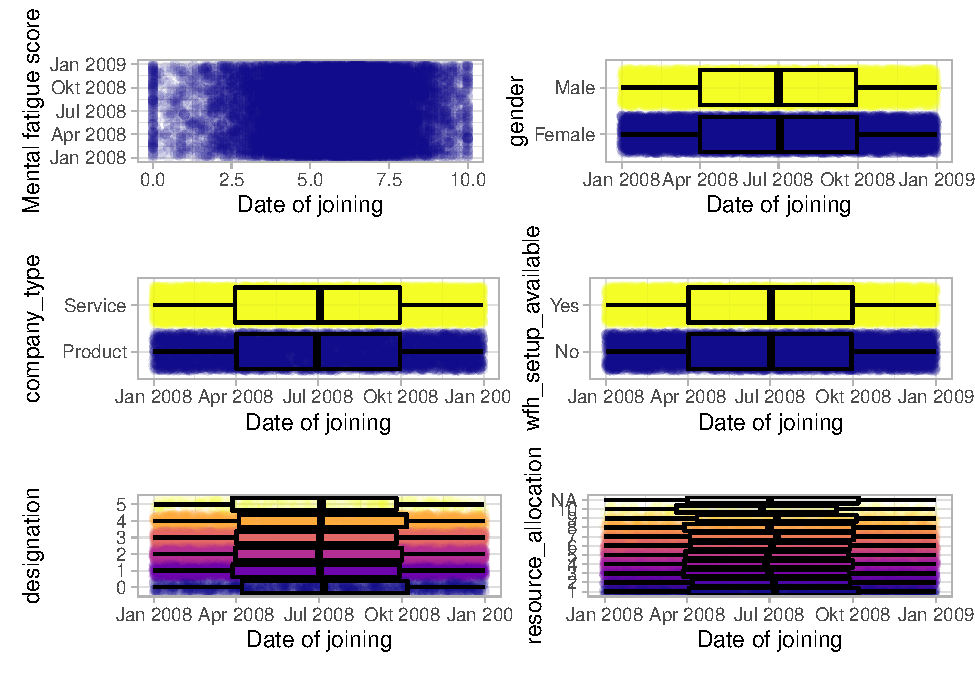
\includegraphics[width=0.9\linewidth]{boosting_methods_files/figure-latex/ggpairs-1}

No major relationship can be detected here.

\hypertarget{gender-vs.-the-remaining}{%
\subsubsection{Gender vs.~the remaining}\label{gender-vs.-the-remaining}}

\textbf{Contingency tables for the comparison of two binary features:}

\begin{Shaded}
\begin{Highlighting}[]
\CommentTok{\# Gender vs Company type}
\FunctionTok{table}\NormalTok{(burnout\_train}\SpecialCharTok{$}\NormalTok{gender, burnout\_train}\SpecialCharTok{$}\NormalTok{company\_type)}
\end{Highlighting}
\end{Shaded}

\begin{verbatim}
##         
##          Product Service
##   Female    3086    5953
##   Male      2916    5345
\end{verbatim}

No huge tendency visible.

\begin{Shaded}
\begin{Highlighting}[]
\CommentTok{\# Gender vs Work from home setup}
\FunctionTok{table}\NormalTok{(burnout\_train}\SpecialCharTok{$}\NormalTok{gender, burnout\_train}\SpecialCharTok{$}\NormalTok{wfh\_setup\_available)}
\end{Highlighting}
\end{Shaded}

\begin{verbatim}
##         
##            No  Yes
##   Female 3878 5161
##   Male   4104 4157
\end{verbatim}

Slightly more women have a work from home setup available.

\textbf{Now the ordinal variables:}

\includegraphics{boosting_methods_files/figure-latex/unnamed-chunk-29-1.pdf}

It has to be noted again that female and male emplyees are almost equally represented in the data set. Thus one can see from the above plot that the biggest difference in distribution is for the levels 1 and 4 with opposing effects. While male employees more often have a quite high designation of 4 females are the much more frequent employee with designation level 1.

\includegraphics{boosting_methods_files/figure-latex/unnamed-chunk-30-1.pdf}

Here a major shift in distribution is visible towards men getting more resources allocated to them. This reflects the society that still promotes men much more often to high paying jobs that most often come with resource responsibility.

\textbf{Now the mental fatigue score:}

\includegraphics{boosting_methods_files/figure-latex/unnamed-chunk-31-1.pdf}

This is of course very similar to the main effect of the \texttt{gender} variable as the outcome and the feature \texttt{mental\_fatigue\_score} are highly linearly correlated.

\hypertarget{company-type-vs.-the-remaining}{%
\subsubsection{Company type vs.~the remaining}\label{company-type-vs.-the-remaining}}

\begin{Shaded}
\begin{Highlighting}[]
\CommentTok{\# Company type vs Work from home setup}
\FunctionTok{table}\NormalTok{(burnout\_train}\SpecialCharTok{$}\NormalTok{company\_type, burnout\_train}\SpecialCharTok{$}\NormalTok{wfh\_setup\_available)}
\end{Highlighting}
\end{Shaded}

\begin{verbatim}
##          
##             No  Yes
##   Product 2805 3197
##   Service 5177 6121
\end{verbatim}

No notable trend.

\includegraphics{boosting_methods_files/figure-latex/unnamed-chunk-33-1.pdf}

No trend here either.

\hypertarget{work-from-home-setup-vs.-the-remaining}{%
\subsubsection{Work from home setup vs.~the remaining}\label{work-from-home-setup-vs.-the-remaining}}

\includegraphics{boosting_methods_files/figure-latex/unnamed-chunk-34-1.pdf}

A work from home setup is way more often available for employees with a lower designation (\(\leq 2\)).

\includegraphics{boosting_methods_files/figure-latex/unnamed-chunk-35-1.pdf}

The same structure as in the previous comparison is visible here again. Employees with a lower amount of resources allocated to them have more often a work from home setup available. This could be due to the fewer responsibilities they have in the business.

\includegraphics{boosting_methods_files/figure-latex/unnamed-chunk-36-1.pdf}

Again this is of course very similar to the main effect of the \texttt{wfh\_setup\_available} variable as the outcome and the feature \texttt{mental\_fatigue\_score} are highly linearly correlated.

\hypertarget{designation-vs-the-remaining}{%
\subsubsection{Designation vs the remaining}\label{designation-vs-the-remaining}}

\includegraphics{boosting_methods_files/figure-latex/unnamed-chunk-37-1.pdf}

Here a strong quite linear relationship is visible. This is sensible as often more resource responsibility is given to employees with high designation.

The last two relationships will be omitted here as both for the variable \texttt{designation} as well as for \texttt{resource\_allocation} the comparison with \texttt{mental\_fatigue\_score} will be very similar to the main effect of the two variables. This comes again from the high correlation of the latter with the outcome.

Overall some stronger and mainly less strong relationships between the predictors could be detected. Not like in ordinary least squares regression for gradient tree boosting no decorrelation and normalization of the features is needed. But before one fixes the pre-processing one can try to extract some more information from some features through some feature engineering.

\hypertarget{some-feature-engineering}{%
\subsection{Some feature engineering}\label{some-feature-engineering}}

The only variable that allows for reasonable feature engineering is the date of joining predictor. One can try to extract some underlying patterns and see if an effect on the outcome is visible.

First extract the day of the week:

\includegraphics{boosting_methods_files/figure-latex/unnamed-chunk-38-1.pdf}

No main effect is visible here. So try the month next.

\includegraphics{boosting_methods_files/figure-latex/unnamed-chunk-39-1.pdf}

Again no main effect is visible.

Nevertheless one can include those two variables into the model because as mentioned before tree-based models actually perform a feature selection at each split. So including these just comes at a small computational cost. This minimal pre-processing that is needed when dealing with tree-based models is actually one of its biggest strengths. It is very robust against any kind of weird selection of features with different scales for example. This is one of the reasons, beside the strong predictive power, for the heavy use of such models in data mining applications.\citep{elements}

\hypertarget{create-the-recipe}{%
\subsection{Create the recipe}\label{create-the-recipe}}

A recipe is an object that defines a series of steps for data pre-processing and feature engineering.

\begin{Shaded}
\begin{Highlighting}[]
\DocumentationTok{\#\#\# recipe for xgboost (nominal variables must be dummy variables)}
\CommentTok{\# define outcome, predictors and training data set}
\NormalTok{burnout\_rec\_boost }\OtherTok{\textless{}{-}} \FunctionTok{recipe}\NormalTok{(burn\_rate }\SpecialCharTok{\textasciitilde{}}\NormalTok{ date\_of\_joining }\SpecialCharTok{+}\NormalTok{ gender }\SpecialCharTok{+}
\NormalTok{                            company\_type }\SpecialCharTok{+}\NormalTok{ wfh\_setup\_available }\SpecialCharTok{+}
\NormalTok{                            designation }\SpecialCharTok{+}\NormalTok{ resource\_allocation }\SpecialCharTok{+}
\NormalTok{                            mental\_fatigue\_score,}
                            \AttributeTok{data =}\NormalTok{ burnout\_train) }\SpecialCharTok{\%\textgreater{}\%}
  \CommentTok{\# extract the date features day of the week and month}
  \FunctionTok{step\_date}\NormalTok{(date\_of\_joining, }\AttributeTok{features =} \FunctionTok{c}\NormalTok{(}\StringTok{"dow"}\NormalTok{, }\StringTok{"month"}\NormalTok{)) }\SpecialCharTok{\%\textgreater{}\%}
  \CommentTok{\# dummify all nominal features}
  \FunctionTok{step\_dummy}\NormalTok{(}\FunctionTok{all\_nominal}\NormalTok{()) }\SpecialCharTok{\%\textgreater{}\%}
  \CommentTok{\# encode the date as integers}
  \FunctionTok{step\_mutate}\NormalTok{(}\AttributeTok{date\_of\_joining =} \FunctionTok{as.integer}\NormalTok{(date\_of\_joining))}

\DocumentationTok{\#\#\# recipe for xgboost (nominal variables must be dummy variables)}
\DocumentationTok{\#\#\# HERE the TRANSFORMED target}
\NormalTok{burnout\_rec\_boost\_trans }\OtherTok{\textless{}{-}} \FunctionTok{recipe}\NormalTok{(burn\_rate\_trans }\SpecialCharTok{\textasciitilde{}}\NormalTok{ date\_of\_joining }\SpecialCharTok{+}\NormalTok{ gender }\SpecialCharTok{+}
\NormalTok{                            company\_type }\SpecialCharTok{+}\NormalTok{ wfh\_setup\_available }\SpecialCharTok{+}
\NormalTok{                            designation }\SpecialCharTok{+}\NormalTok{ resource\_allocation }\SpecialCharTok{+}
\NormalTok{                            mental\_fatigue\_score,}
                            \AttributeTok{data =}\NormalTok{ burnout\_train) }\SpecialCharTok{\%\textgreater{}\%}
  \CommentTok{\# extract the date features day of the week and month}
  \FunctionTok{step\_date}\NormalTok{(date\_of\_joining, }\AttributeTok{features =} \FunctionTok{c}\NormalTok{(}\StringTok{"dow"}\NormalTok{, }\StringTok{"month"}\NormalTok{)) }\SpecialCharTok{\%\textgreater{}\%}
  \CommentTok{\# dummify all nominal features}
  \FunctionTok{step\_dummy}\NormalTok{(}\FunctionTok{all\_nominal}\NormalTok{()) }\SpecialCharTok{\%\textgreater{}\%}
  \CommentTok{\# encode the date as integers}
  \FunctionTok{step\_mutate}\NormalTok{(}\AttributeTok{date\_of\_joining =} \FunctionTok{as.integer}\NormalTok{(date\_of\_joining))}

\DocumentationTok{\#\#\# recipe for a random forest model for comparison (no dummy encoding needed)}
\CommentTok{\# same as above without dummification but here the na\textquotesingle{}s have to be}
\CommentTok{\# imputed (here via knn)}
\NormalTok{burnout\_rec\_rf }\OtherTok{\textless{}{-}} \FunctionTok{recipe}\NormalTok{(burn\_rate }\SpecialCharTok{\textasciitilde{}}\NormalTok{ date\_of\_joining }\SpecialCharTok{+}\NormalTok{ gender }\SpecialCharTok{+}
\NormalTok{                         company\_type }\SpecialCharTok{+}\NormalTok{ wfh\_setup\_available }\SpecialCharTok{+}
\NormalTok{                         designation }\SpecialCharTok{+}\NormalTok{ resource\_allocation }\SpecialCharTok{+}
\NormalTok{                         mental\_fatigue\_score,}
                         \AttributeTok{data =}\NormalTok{ burnout\_train) }\SpecialCharTok{\%\textgreater{}\%}
  \FunctionTok{step\_string2factor}\NormalTok{(}\FunctionTok{all\_nominal}\NormalTok{()) }\SpecialCharTok{\%\textgreater{}\%}
  \FunctionTok{step\_impute\_knn}\NormalTok{(resource\_allocation, }\AttributeTok{neighbors =} \DecValTok{5}\NormalTok{) }\SpecialCharTok{\%\textgreater{}\%}
  \FunctionTok{step\_impute\_knn}\NormalTok{(mental\_fatigue\_score, }\AttributeTok{neighbors =} \DecValTok{5}\NormalTok{) }\SpecialCharTok{\%\textgreater{}\%}
  \FunctionTok{step\_date}\NormalTok{(date\_of\_joining, }\AttributeTok{features =} \FunctionTok{c}\NormalTok{(}\StringTok{"dow"}\NormalTok{, }\StringTok{"month"}\NormalTok{)) }\SpecialCharTok{\%\textgreater{}\%}
  \FunctionTok{step\_mutate}\NormalTok{(}\AttributeTok{date\_of\_joining =} \FunctionTok{as.integer}\NormalTok{(date\_of\_joining))}
\end{Highlighting}
\end{Shaded}

\hypertarget{insurence-data}{%
\section{Insurence data}\label{insurence-data}}

The insurance data set is part of the book \emph{Machine Learning with R} by Brett Lantz. It can be downloaded here:
\url{https://raw.githubusercontent.com/stedy/Machine-Learning-with-R-datasets/master/insurance.csv}

\begin{Shaded}
\begin{Highlighting}[]
\CommentTok{\# load the data}
\NormalTok{insurance\_data }\OtherTok{\textless{}{-}} \FunctionTok{read\_csv}\NormalTok{(}\StringTok{"\_data/insurance.csv"}\NormalTok{)}
\end{Highlighting}
\end{Shaded}

\hypertarget{train-test-split-1}{%
\subsection{Train-test split}\label{train-test-split-1}}

\begin{Shaded}
\begin{Highlighting}[]
\FunctionTok{set.seed}\NormalTok{(}\DecValTok{2}\NormalTok{)}
\NormalTok{ins\_split }\OtherTok{\textless{}{-}}\NormalTok{ rsample}\SpecialCharTok{::}\FunctionTok{initial\_split}\NormalTok{(insurance\_data, }\AttributeTok{prop =} \FloatTok{0.80}\NormalTok{)}
\NormalTok{ins\_train }\OtherTok{\textless{}{-}}\NormalTok{ rsample}\SpecialCharTok{::}\FunctionTok{training}\NormalTok{(ins\_split)}
\NormalTok{ins\_test  }\OtherTok{\textless{}{-}}\NormalTok{ rsample}\SpecialCharTok{::}\FunctionTok{testing}\NormalTok{(ins\_split)}
\end{Highlighting}
\end{Shaded}

The training data set contains 1070 rows and 7 variables.

The test data set contains 268 observations and naturally also 7 variables.

\hypertarget{a-general-overview}{%
\subsection{A general overview}\label{a-general-overview}}

A general visualization of the whole data set in order to detect missing values.

\includegraphics{boosting_methods_files/figure-latex/visdatIns-1.pdf}

So there are no missing values!

\hypertarget{what-about-the-outcome}{%
\subsection{What about the outcome?}\label{what-about-the-outcome}}

\texttt{charges}: Individual medical costs billed by health insurance.

The five point summary below shows that the no invalid values i.e.~negative ones are in the data.

\begin{verbatim}
##    Min. 1st Qu.  Median    Mean 3rd Qu.    Max. 
##    1122    4741    9289   13316   16640   62593
\end{verbatim}

Now the distribution of the outcome.

\includegraphics{boosting_methods_files/figure-latex/unnamed-chunk-43-1.pdf}

Not like the \texttt{burn\_rate} previously this target distribution is not at all symmetrical but highly right skewed. A natural thing to do would be a log transformation of the outcome. The resulting \texttt{log10\_charges} outcome variable is shown below.

\includegraphics{boosting_methods_files/figure-latex/unnamed-chunk-45-1.pdf}

Although such a transformation of the outcome variable is not needed for tree-based modeling it can make the job of the algorithm somewhat easier.

\hypertarget{distribution-and-main-effects-of-the-predictors-1}{%
\subsection{Distribution and main effects of the predictors}\label{distribution-and-main-effects-of-the-predictors-1}}

\hypertarget{age}{%
\subsubsection{Age}\label{age}}

\texttt{age}: The age of the insurance contractor. This is naturally a continuous variable.

\includegraphics{boosting_methods_files/figure-latex/unnamed-chunk-46-1.pdf}

A wide range of ages is covered. Notably there is a peak at roughly 18 which means that many fresh adults were observed in this data set.

\includegraphics{boosting_methods_files/figure-latex/unnamed-chunk-47-1.pdf}

There seems to be a strong main effect although it does not seem to be linear. The general trend is that older contractors generally accumulate more medical costs. This is very intuitive.

\hypertarget{sex}{%
\subsubsection{Sex}\label{sex}}

\texttt{sex}: The insurance contractors gender. Here either female or male. This means it is a binary variable and will be treated as such.

\begin{Shaded}
\begin{Highlighting}[]
\FunctionTok{summary}\NormalTok{(}\FunctionTok{as.factor}\NormalTok{(ins\_train}\SpecialCharTok{$}\NormalTok{sex))}
\end{Highlighting}
\end{Shaded}

\begin{verbatim}
## female   male 
##    544    526
\end{verbatim}

The classes are very well balanced. Now the main effect.

\includegraphics{boosting_methods_files/figure-latex/unnamed-chunk-49-1.pdf}

No notable difference can be detected here.

\hypertarget{body-mass-index}{%
\subsubsection{Body mass index}\label{body-mass-index}}

\texttt{bmi}: The body mass index is providing an understanding of the body composition. It is a ratio composed out of the weight which is divided by the height \(\frac{kg}{m^2}\). Ideally the ratio is between 18.5 and 24.9. The variable is obviously a continuous variable.

\includegraphics{boosting_methods_files/figure-latex/unnamed-chunk-50-1.pdf}

The distribution is bell-shaped and symmetrical roughly around a bmi of 30 which is above the ideal range. Actually only a small amount of the data falls into the normal range here. Moreover the right tail is heavier than the left one. Now a look at the main effect of the variable.

\includegraphics{boosting_methods_files/figure-latex/unnamed-chunk-51-1.pdf}

With some fantasy one can grasp some non-linear patterns on the right side of the plot but beside that no strong main effect is visible here.

\hypertarget{number-of-children}{%
\subsubsection{Number of children}\label{number-of-children}}

\texttt{children}: The number of children or dependents covered by the health insurance.

\begin{Shaded}
\begin{Highlighting}[]
\CommentTok{\# unique values of the feature}
\FunctionTok{unique}\NormalTok{(ins\_train}\SpecialCharTok{$}\NormalTok{children)}
\end{Highlighting}
\end{Shaded}

\begin{verbatim}
## [1] 0 1 2 3 4 5
\end{verbatim}

This could be treated as categorical but as there is a natural ordering it will be encoded by the integers so the treatment is like the one of a continuous feature.

\includegraphics{boosting_methods_files/figure-latex/unnamed-chunk-53-1.pdf}

As one would also think the more children the lower the number of observed values. Especially the numbers greater than 3 are not well represented. If encoded by one-hot-encoding one would have to think about removing these then near-zero-variance variables. But as they will be encoded in a continuous way this is no problem at all. A look at the main effects can now strengthen or weaken this hypothesis of a natural ordering.

\includegraphics{boosting_methods_files/figure-latex/unnamed-chunk-54-1.pdf}

This plot is quite similar to the main effect plot for the \texttt{age} feature. As most likely (will be checked later) the age is positively correlated with the number of children one can observe a rise of the minimal observed charges towards a greater amount of children. The upper two boxplots are built with just a few observations so they should not be interpreted in great detail. Overall there seems to be some kind of main effect.

\hypertarget{smoking}{%
\subsubsection{Smoking}\label{smoking}}

\texttt{smoker}: Is the contractor smoking? Of course a binary variable.

\begin{Shaded}
\begin{Highlighting}[]
\FunctionTok{summary}\NormalTok{(}\FunctionTok{as.factor}\NormalTok{(ins\_train}\SpecialCharTok{$}\NormalTok{smoker))}
\end{Highlighting}
\end{Shaded}

\begin{verbatim}
##  no yes 
## 849 221
\end{verbatim}

The classes are not balanced but the class of the smokers is still represented with a good amount of observations. Now a look at the main effect.

\includegraphics{boosting_methods_files/figure-latex/unnamed-chunk-56-1.pdf}

This main effect is as drastic as it is intuitive. Smoking seems to definitely increases the charges. This means that this variable has probably a lot of predictive power.

\hypertarget{region}{%
\subsubsection{Region}\label{region}}

\texttt{region}: The beneficiary's residential area in the US. Either northeast, southeast, southwest or northwest. This definitely is a categorical variable.

\includegraphics{boosting_methods_files/figure-latex/unnamed-chunk-57-1.pdf}

The four regions are balanced. Now to the main effect.

\includegraphics{boosting_methods_files/figure-latex/unnamed-chunk-58-1.pdf}

No important main effect is detectable from this plot.

\hypertarget{relationships-between-the-predictors-1}{%
\subsection{Relationships between the predictors}\label{relationships-between-the-predictors-1}}

\hypertarget{age-vs-the-others}{%
\subsubsection{Age vs the others}\label{age-vs-the-others}}

First the continuous one: \texttt{bmi}

\includegraphics{boosting_methods_files/figure-latex/unnamed-chunk-59-1.pdf}

No relationship detectable. The pearson correlation is with 0.089 also low.

\includegraphics{boosting_methods_files/figure-latex/unnamed-chunk-61-1.pdf}

The most interesting take away from these four plots is that the hypothesis about the age of the contractors with children seem to be okish except for the ones with more than 3 children. But again this counterintuitive behavior could also be due to the few samples. At this point one might think about encoding the children variable as a categorical but in the following it will be left continuous.

\hypertarget{sex-vs-the-remaining}{%
\subsubsection{Sex vs the remaining}\label{sex-vs-the-remaining}}

\includegraphics{boosting_methods_files/figure-latex/unnamed-chunk-62-1.pdf}

No notable differences.

Contingency table for the binary variable \texttt{smoker}:

\begin{Shaded}
\begin{Highlighting}[]
\CommentTok{\# sex vs smoker}
\FunctionTok{table}\NormalTok{(ins\_train}\SpecialCharTok{$}\NormalTok{sex, ins\_train}\SpecialCharTok{$}\NormalTok{smoker)}
\end{Highlighting}
\end{Shaded}

\begin{verbatim}
##         
##           no yes
##   female 448  96
##   male   401 125
\end{verbatim}

Slightly more men smoke but the difference is smallish.

\hypertarget{bmi-vs-the-remaining}{%
\subsubsection{BMI vs the remaining}\label{bmi-vs-the-remaining}}

\includegraphics{boosting_methods_files/figure-latex/unnamed-chunk-64-1.pdf}

The most notable fact here is that southeast of the US seems to be a little more overweight than the rest.

\hypertarget{children-vs-the-remaining}{%
\subsubsection{Children vs the remaining}\label{children-vs-the-remaining}}

\includegraphics{boosting_methods_files/figure-latex/unnamed-chunk-65-1.pdf}

In relative terms actually the contractors with three children smoke the most but the other levels seem quite balanced.

\includegraphics{boosting_methods_files/figure-latex/unnamed-chunk-66-1.pdf}

Here no trend is visible.

\hypertarget{smoker-vs-region}{%
\subsubsection{Smoker vs Region}\label{smoker-vs-region}}

\includegraphics{boosting_methods_files/figure-latex/unnamed-chunk-67-1.pdf}

So the southeast is not only the most overweight region but also the one with the most smokers in relative terms.

This concludes the tour of the pairwise relationships. Of course such an in detail look at all pairwise relationships for both data sets was only possible because there are quite few predictors and is not always needed in this extend. Besides a crystal clear understanding of the data one sees that there is not much room left for feature engineering for the insurance data set. Thus one can go on and define the recipe.

\hypertarget{create-the-recipe-1}{%
\subsection{Create the recipe}\label{create-the-recipe-1}}

Transformations on the outcome variable are not good practice within a recipe thus this will be done now before hand by adding a new feature i.e.~\texttt{log10\_charges} to the train and test data set.

\begin{Shaded}
\begin{Highlighting}[]
\CommentTok{\# add the log transformed outcome variable to the data}
\NormalTok{ins\_train}\SpecialCharTok{$}\NormalTok{log10\_charges }\OtherTok{\textless{}{-}} \FunctionTok{log10}\NormalTok{(ins\_train}\SpecialCharTok{$}\NormalTok{charges)}
\NormalTok{ins\_test}\SpecialCharTok{$}\NormalTok{log10\_charges }\OtherTok{\textless{}{-}} \FunctionTok{log10}\NormalTok{(ins\_test}\SpecialCharTok{$}\NormalTok{charges)}
\end{Highlighting}
\end{Shaded}

\begin{Shaded}
\begin{Highlighting}[]
\DocumentationTok{\#\#\# recipe for xgboost (nominal variables must be dummy variables)}
\CommentTok{\# define outcome, predictors and training data set}
\NormalTok{ins\_rec\_boost }\OtherTok{\textless{}{-}} \FunctionTok{recipe}\NormalTok{(log10\_charges }\SpecialCharTok{\textasciitilde{}}\NormalTok{ age }\SpecialCharTok{+}\NormalTok{ sex }\SpecialCharTok{+}
\NormalTok{                            bmi }\SpecialCharTok{+}\NormalTok{ children }\SpecialCharTok{+}
\NormalTok{                            smoker }\SpecialCharTok{+}\NormalTok{ region,}
                            \AttributeTok{data =}\NormalTok{ ins\_train) }\SpecialCharTok{\%\textgreater{}\%}
  \CommentTok{\# dummify all nominal features (sex, smoker, region)}
  \FunctionTok{step\_dummy}\NormalTok{(}\FunctionTok{all\_nominal}\NormalTok{())}

\DocumentationTok{\#\#\# recipe for a random forest model for comparison (no dummy encoding needed)}
\CommentTok{\# same as above without dummification }
\NormalTok{ins\_rec\_rf }\OtherTok{\textless{}{-}} \FunctionTok{recipe}\NormalTok{(log10\_charges }\SpecialCharTok{\textasciitilde{}}\NormalTok{ age }\SpecialCharTok{+}\NormalTok{ sex }\SpecialCharTok{+}
\NormalTok{                         bmi }\SpecialCharTok{+}\NormalTok{ children }\SpecialCharTok{+}
\NormalTok{                         smoker }\SpecialCharTok{+}\NormalTok{ region,}
                         \AttributeTok{data =}\NormalTok{ ins\_train)}
\end{Highlighting}
\end{Shaded}

Having now all the recipes ready one can proceed with modeling. Finally!

\hypertarget{modeling}{%
\chapter{Let's boost the models}\label{modeling}}

Beside the XGBoost model also a random forest model will be fitted here for comparison. The whole modeling approach and procedure is closely following the principles that are outlined in the \textbf{great} book \emph{Tidy modeling with R} by Max Kuhn and Julia Silge.

For the modeling three additional packages are required.\citep{xgboost_package, ranger_package, vipPack}

\begin{Shaded}
\begin{Highlighting}[]
\FunctionTok{library}\NormalTok{(xgboost) }\CommentTok{\# for the xgboost model}
\FunctionTok{library}\NormalTok{(ranger) }\CommentTok{\# for the random forest model}
\CommentTok{\# + the vip package but it will not be loaded into}
\CommentTok{\# the namespace}
\end{Highlighting}
\end{Shaded}

For parallel computations the \texttt{doParallel} package is used.\citep{doParallel_package}
This is most useful for the tuning part.

\begin{Shaded}
\begin{Highlighting}[]
\FunctionTok{library}\NormalTok{(doParallel)}

\CommentTok{\# Create a cluster object and then register: }
\NormalTok{cl }\OtherTok{\textless{}{-}} \FunctionTok{makePSOCKcluster}\NormalTok{(}\DecValTok{2}\NormalTok{)}
\FunctionTok{registerDoParallel}\NormalTok{(cl)}
\end{Highlighting}
\end{Shaded}

First one has to set a \textbf{metric} for the evaluation of the final performance. As one knows from the EDA that not a lot of outliers are present in the data one can leave the default for XGBoost as the optimization metric for regression which is the root mean squared error (RMSE) which basically corresponds to the \(L_2\) loss. Besides also the mean average error (MAE) which is kind of the \(L_1\) norm will be covered but the optimization and tuning will focus on the RMSE.

\hypertarget{burnout-data-1}{%
\section{Burnout data}\label{burnout-data-1}}

\hypertarget{baseline-models}{%
\subsection{Baseline models}\label{baseline-models}}

The first thing is to set up the trivial \textbf{baseline models}.

\begin{Shaded}
\begin{Highlighting}[]
\CommentTok{\# the trivial intercept only model:}
\NormalTok{bout\_predict\_trivial\_mean }\OtherTok{\textless{}{-}} \ControlFlowTok{function}\NormalTok{(new\_data) \{}
  \FunctionTok{rep}\NormalTok{(}\FunctionTok{mean}\NormalTok{(burnout\_train}\SpecialCharTok{$}\NormalTok{burn\_rate), }\FunctionTok{nrow}\NormalTok{(new\_data))}
\NormalTok{\}}

\CommentTok{\# the trivial scoring of mental fatigue score (if missing intercept model)}
\NormalTok{bout\_predict\_trivial\_mfs }\OtherTok{\textless{}{-}} \ControlFlowTok{function}\NormalTok{(new\_data) \{}
  \CommentTok{\# these two scoring parameters are correspondint to the }
  \CommentTok{\# simple linear regression model containing only one predictor}
  \CommentTok{\# i.e. mfs}
\NormalTok{  pred }\OtherTok{\textless{}{-}}\NormalTok{ new\_data[[}\StringTok{"mental\_fatigue\_score"}\NormalTok{]] }\SpecialCharTok{*} \FloatTok{0.097} \SpecialCharTok{{-}} \FloatTok{0.1}
\NormalTok{  pred[}\FunctionTok{is.na}\NormalTok{(pred)] }\OtherTok{\textless{}{-}} \FunctionTok{mean}\NormalTok{(burnout\_train}\SpecialCharTok{$}\NormalTok{burn\_rate)}
\NormalTok{  pred}
\NormalTok{\}}
\end{Highlighting}
\end{Shaded}

The predictions of these baseline models on the test data set will be compared with the predictions of the tree-based models that will be constructed.

\hypertarget{model-specification}{%
\subsection{Model specification}\label{model-specification}}

\begin{Shaded}
\begin{Highlighting}[]
\CommentTok{\# Models:}

\CommentTok{\# Random forest model for comparison}
\NormalTok{bout\_rf\_model }\OtherTok{\textless{}{-}} \FunctionTok{rand\_forest}\NormalTok{(}\AttributeTok{trees =} \FunctionTok{tune}\NormalTok{(),}
                             \AttributeTok{mtry =} \FunctionTok{tune}\NormalTok{()) }\SpecialCharTok{\%\textgreater{}\%} 
  \FunctionTok{set\_engine}\NormalTok{(}\StringTok{"ranger"}\NormalTok{) }\SpecialCharTok{\%\textgreater{}\%} 
  \FunctionTok{set\_mode}\NormalTok{(}\StringTok{"regression"}\NormalTok{)}

\CommentTok{\# XGBoost model }
\NormalTok{bout\_boost\_model }\OtherTok{\textless{}{-}} \FunctionTok{boost\_tree}\NormalTok{(}\AttributeTok{trees =} \FunctionTok{tune}\NormalTok{(),}
                               \AttributeTok{learn\_rate =} \FunctionTok{tune}\NormalTok{(),}
                               \AttributeTok{loss\_reduction =} \FunctionTok{tune}\NormalTok{(),}
                               \AttributeTok{tree\_depth =} \FunctionTok{tune}\NormalTok{(),}
                               \AttributeTok{mtry =} \FunctionTok{tune}\NormalTok{(),}
                               \AttributeTok{sample\_size =} \FunctionTok{tune}\NormalTok{(),}
                               \AttributeTok{stop\_iter =} \DecValTok{10}\NormalTok{) }\SpecialCharTok{\%\textgreater{}\%}
  \FunctionTok{set\_engine}\NormalTok{(}\StringTok{"xgboost"}\NormalTok{) }\SpecialCharTok{\%\textgreater{}\%} 
  \FunctionTok{set\_mode}\NormalTok{(}\StringTok{"regression"}\NormalTok{)}
\end{Highlighting}
\end{Shaded}

\begin{Shaded}
\begin{Highlighting}[]
\CommentTok{\# Workflows: model + recipe}

\CommentTok{\# Random Forest workflow}
\NormalTok{bout\_rf\_wflow }\OtherTok{\textless{}{-}}
  \FunctionTok{workflow}\NormalTok{() }\SpecialCharTok{\%\textgreater{}\%}
  \FunctionTok{add\_model}\NormalTok{(bout\_rf\_model) }\SpecialCharTok{\%\textgreater{}\%}
  \FunctionTok{add\_recipe}\NormalTok{(burnout\_rec\_rf)}

\CommentTok{\# XGBoost workflow with the untransformed target}
\NormalTok{bout\_boost\_wflow }\OtherTok{\textless{}{-}}
  \FunctionTok{workflow}\NormalTok{() }\SpecialCharTok{\%\textgreater{}\%}
  \FunctionTok{add\_model}\NormalTok{(bout\_boost\_model) }\SpecialCharTok{\%\textgreater{}\%}
  \FunctionTok{add\_recipe}\NormalTok{(burnout\_rec\_boost)}

\CommentTok{\# XGBoost workflow with the transformed target (empirical logit)}
\NormalTok{bout\_boost\_wflow\_trans }\OtherTok{\textless{}{-}}
  \FunctionTok{workflow}\NormalTok{() }\SpecialCharTok{\%\textgreater{}\%}
  \FunctionTok{add\_model}\NormalTok{(bout\_boost\_model) }\SpecialCharTok{\%\textgreater{}\%}
  \FunctionTok{add\_recipe}\NormalTok{(burnout\_rec\_boost\_trans)}
\end{Highlighting}
\end{Shaded}

\hypertarget{tuning}{%
\subsection{Tuning}\label{tuning}}

For the hyperparameter tuning one needs validation sets to monitor the models on unseen data. To do this 5-fold cross validation (CV) is used here.

\begin{Shaded}
\begin{Highlighting}[]
\CommentTok{\# Create Resampling object}
\FunctionTok{set.seed}\NormalTok{(}\DecValTok{2}\NormalTok{)}
\NormalTok{burnout\_folds }\OtherTok{\textless{}{-}} \FunctionTok{vfold\_cv}\NormalTok{(burnout\_train, }\AttributeTok{v =} \DecValTok{5}\NormalTok{)}
\end{Highlighting}
\end{Shaded}

Now adjust or check the hyperparameter ranges that the tuning will use. First the Random forest model.

\begin{Shaded}
\begin{Highlighting}[]
\CommentTok{\# Have a look at the hyperparameters that have to be tuned and finalize them}
\NormalTok{bout\_rf\_params }\OtherTok{\textless{}{-}}\NormalTok{ bout\_rf\_wflow }\SpecialCharTok{\%\textgreater{}\%}
  \FunctionTok{parameters}\NormalTok{()}

\NormalTok{bout\_rf\_params }
\end{Highlighting}
\end{Shaded}

\begin{verbatim}
## Collection of 2 parameters for tuning
## 
##  identifier  type    object
##        mtry  mtry nparam[?]
##       trees trees nparam[+]
## 
## Model parameters needing finalization:
##    # Randomly Selected Predictors ('mtry')
## 
## See `?dials::finalize` or `?dials::update.parameters` for more information.
\end{verbatim}

This shows that the \texttt{mtry} hyperparameter has to be adjusted depending on the data. Moreover with the \texttt{dials::update} function one can manually set the ranges that should be used for tuning.

\begin{Shaded}
\begin{Highlighting}[]
\CommentTok{\# default range for tuning is 1 up to 2000 for the trees argument}
\CommentTok{\# set the lower bound of the range to 100. Then finalize the}
\CommentTok{\# parameters using the training data.}
\NormalTok{bout\_rf\_params }\OtherTok{\textless{}{-}}\NormalTok{ bout\_rf\_params }\SpecialCharTok{\%\textgreater{}\%}
  \FunctionTok{update}\NormalTok{(}\AttributeTok{trees =} \FunctionTok{trees}\NormalTok{(}\FunctionTok{c}\NormalTok{(}\DecValTok{100}\NormalTok{, }\DecValTok{2000}\NormalTok{))) }\SpecialCharTok{\%\textgreater{}\%}
  \FunctionTok{finalize}\NormalTok{(burnout\_train)}
\NormalTok{bout\_rf\_params}
\end{Highlighting}
\end{Shaded}

\begin{verbatim}
## Collection of 2 parameters for tuning
## 
##  identifier  type    object
##        mtry  mtry nparam[+]
##       trees trees nparam[+]
\end{verbatim}

\begin{Shaded}
\begin{Highlighting}[]
\NormalTok{bout\_rf\_params }\SpecialCharTok{\%\textgreater{}\%} \FunctionTok{pull\_dials\_object}\NormalTok{(}\StringTok{"mtry"}\NormalTok{)}
\end{Highlighting}
\end{Shaded}

\begin{verbatim}
## # Randomly Selected Predictors (quantitative)
## Range: [1, 10]
\end{verbatim}

\begin{Shaded}
\begin{Highlighting}[]
\NormalTok{bout\_rf\_params }\SpecialCharTok{\%\textgreater{}\%} \FunctionTok{pull\_dials\_object}\NormalTok{(}\StringTok{"trees"}\NormalTok{)}
\end{Highlighting}
\end{Shaded}

\begin{verbatim}
## # Trees (quantitative)
## Range: [100, 2000]
\end{verbatim}

Now this parameter object is ready for tuning and the same steps have to be performed on the main boosting workflow. The parameter set for the untransformed target can then also be used for the transformed one.

\begin{Shaded}
\begin{Highlighting}[]
\NormalTok{bout\_boost\_params }\OtherTok{\textless{}{-}}\NormalTok{ bout\_boost\_wflow }\SpecialCharTok{\%\textgreater{}\%}
  \FunctionTok{parameters}\NormalTok{()}

\NormalTok{bout\_boost\_params }
\end{Highlighting}
\end{Shaded}

\begin{verbatim}
## Collection of 6 parameters for tuning
## 
##      identifier           type    object
##            mtry           mtry nparam[?]
##           trees          trees nparam[+]
##      tree_depth     tree_depth nparam[+]
##      learn_rate     learn_rate nparam[+]
##  loss_reduction loss_reduction nparam[+]
##     sample_size    sample_size nparam[+]
## 
## Model parameters needing finalization:
##    # Randomly Selected Predictors ('mtry')
## 
## See `?dials::finalize` or `?dials::update.parameters` for more information.
\end{verbatim}

\begin{Shaded}
\begin{Highlighting}[]
\CommentTok{\# first a look at the default ranges}
\FunctionTok{trees}\NormalTok{()}
\end{Highlighting}
\end{Shaded}

\begin{verbatim}
## # Trees (quantitative)
## Range: [1, 2000]
\end{verbatim}

\begin{Shaded}
\begin{Highlighting}[]
\FunctionTok{tree\_depth}\NormalTok{()}
\end{Highlighting}
\end{Shaded}

\begin{verbatim}
## Tree Depth (quantitative)
## Range: [1, 15]
\end{verbatim}

\begin{Shaded}
\begin{Highlighting}[]
\FunctionTok{learn\_rate}\NormalTok{()}
\end{Highlighting}
\end{Shaded}

\begin{verbatim}
## Learning Rate (quantitative)
## Transformer:  log-10 
## Range (transformed scale): [-10, -1]
\end{verbatim}

\begin{Shaded}
\begin{Highlighting}[]
\FunctionTok{loss\_reduction}\NormalTok{()}
\end{Highlighting}
\end{Shaded}

\begin{verbatim}
## Minimum Loss Reduction (quantitative)
## Transformer:  log-10 
## Range (transformed scale): [-10, 1.5]
\end{verbatim}

\begin{Shaded}
\begin{Highlighting}[]
\FunctionTok{sample\_size}\NormalTok{()}
\end{Highlighting}
\end{Shaded}

\begin{verbatim}
## # Observations Sampled (quantitative)
## Range: [?, ?]
\end{verbatim}

So \texttt{sample\_size} must also be finalized. Again the lower bound on the number of trees will be raised to 100. The other scales are really sensible and will be left as is.

\begin{Shaded}
\begin{Highlighting}[]
\NormalTok{bout\_boost\_params }\OtherTok{\textless{}{-}}\NormalTok{ bout\_boost\_params }\SpecialCharTok{\%\textgreater{}\%}
  \FunctionTok{update}\NormalTok{(}\AttributeTok{trees =} \FunctionTok{trees}\NormalTok{(}\FunctionTok{c}\NormalTok{(}\DecValTok{100}\NormalTok{, }\DecValTok{2000}\NormalTok{))) }\SpecialCharTok{\%\textgreater{}\%}
  \FunctionTok{finalize}\NormalTok{(burnout\_train)}

\NormalTok{bout\_boost\_params}
\end{Highlighting}
\end{Shaded}

\begin{verbatim}
## Collection of 6 parameters for tuning
## 
##      identifier           type    object
##            mtry           mtry nparam[+]
##           trees          trees nparam[+]
##      tree_depth     tree_depth nparam[+]
##      learn_rate     learn_rate nparam[+]
##  loss_reduction loss_reduction nparam[+]
##     sample_size    sample_size nparam[+]
\end{verbatim}

\begin{Shaded}
\begin{Highlighting}[]
\NormalTok{bout\_boost\_params }\SpecialCharTok{\%\textgreater{}\%}
  \FunctionTok{pull\_dials\_object}\NormalTok{(}\StringTok{"sample\_size"}\NormalTok{)}
\end{Highlighting}
\end{Shaded}

\begin{verbatim}
## Proportion Observations Sampled (quantitative)
## Range: [0.1, 1]
\end{verbatim}

\begin{Shaded}
\begin{Highlighting}[]
\NormalTok{bout\_boost\_params }\SpecialCharTok{\%\textgreater{}\%}
  \FunctionTok{pull\_dials\_object}\NormalTok{(}\StringTok{"mtry"}\NormalTok{)}
\end{Highlighting}
\end{Shaded}

\begin{verbatim}
## # Randomly Selected Predictors (quantitative)
## Range: [1, 10]
\end{verbatim}

\begin{Shaded}
\begin{Highlighting}[]
\CommentTok{\# use the same object for the tuning of the boosted model}
\CommentTok{\# with the transformed target}
\NormalTok{bout\_boost\_params\_trans }\OtherTok{\textless{}{-}}\NormalTok{ bout\_boost\_params}
\end{Highlighting}
\end{Shaded}

Now also these parameter objects are ready to be used. The next step is to define the metrics used for evaluation while tuning.

\begin{Shaded}
\begin{Highlighting}[]
\CommentTok{\# define a metrics set used for evaluation of the hyperparameters}
\NormalTok{regr\_metrics }\OtherTok{\textless{}{-}} \FunctionTok{metric\_set}\NormalTok{(rmse, mae)}
\end{Highlighting}
\end{Shaded}

Now the actual tuning begins. The models will be tuned by a space filling grid search. As one has defined ranges for each parameter one can then use different algorithms to construct a grid of combinations of parameter values that tries to best fill the defined ranges by random sampling also in a high dimensional setting. In the following the function \texttt{tune::grid\_latin\_hypercube} is used for this. So basically one tries out all hyperparameter values for each fold and saves the performance of the performance metrics on the hold out fold. These metrics are then aggregated for each combination and with the resulting estimates of performance one can choose the final set of hyperparameters. The more hyperparameters the model has the more tuning rounds might be needed to refine the grid. Besides the classical grid search there are also iterative methods for tuning. These are mainly good to tune a single hyperparameter at once and not for a bunch of them simultaneously. They will not be used in the following.

The \textbf{random forest model} goes first with the tuning.

Here there are as seen above only two hyperparameters to be tuned thus 30 combinations should suffice.

\begin{Shaded}
\begin{Highlighting}[]
\CommentTok{\# took roughly 30 minutes}
\FunctionTok{system.time}\NormalTok{(\{}
  \FunctionTok{set.seed}\NormalTok{(}\DecValTok{2}\NormalTok{)}
\NormalTok{  bout\_rf\_tune }\OtherTok{\textless{}{-}}\NormalTok{ bout\_rf\_wflow }\SpecialCharTok{\%\textgreater{}\%}
    \FunctionTok{tune\_grid}\NormalTok{(}
      \AttributeTok{resamples =}\NormalTok{  burnout\_folds,}
      \AttributeTok{grid =}\NormalTok{ bout\_rf\_params }\SpecialCharTok{\%\textgreater{}\%}
        \FunctionTok{grid\_latin\_hypercube}\NormalTok{(}\AttributeTok{size =} \DecValTok{30}\NormalTok{, }\AttributeTok{original =} \ConstantTok{FALSE}\NormalTok{),}
      \AttributeTok{metrics =}\NormalTok{ regr\_metrics}
\NormalTok{    )}
\NormalTok{\})}

\CommentTok{\# visualization of the tuning results (snapshot of the output below)}
\FunctionTok{autoplot}\NormalTok{(bout\_rf\_tune) }\SpecialCharTok{+} \FunctionTok{theme\_light}\NormalTok{()}
\CommentTok{\# this functions shows the best combinations wrt the rmse metric of all the}
\CommentTok{\# combinations in the grid}
\FunctionTok{show\_best}\NormalTok{(bout\_rf\_tune, }\AttributeTok{metric =} \StringTok{"rmse"}\NormalTok{)}
\end{Highlighting}
\end{Shaded}

\begin{figure}

{\centering \includegraphics[width=0.7\linewidth]{_pictures/rf_burn_tune_plot} 

}

\caption{Result of a spacefilling grid search for the random forest model.}\label{fig:rfburntuneplot}
\end{figure}

The visualization alongside the best performing results suggest that a value of \texttt{mtry}of 3 and 1000 \texttt{trees} should give good results. Thus one can finalize and fit this model.

\begin{Shaded}
\begin{Highlighting}[]
\NormalTok{final\_bout\_rf\_wflow }\OtherTok{\textless{}{-}} 
\NormalTok{  bout\_rf\_wflow }\SpecialCharTok{\%\textgreater{}\%} 
  \FunctionTok{finalize\_workflow}\NormalTok{(}\FunctionTok{tibble}\NormalTok{(}
    \AttributeTok{trees =} \DecValTok{1000}\NormalTok{,}
    \AttributeTok{mtry =} \DecValTok{3}
\NormalTok{  )) }\SpecialCharTok{\%\textgreater{}\%}
  \FunctionTok{fit}\NormalTok{(burnout\_train)}
\end{Highlighting}
\end{Shaded}

Now the main \textbf{boosting model}.

First tune only the number of trees in order to detect a number of
trees that is `large enough'. Then tune the tree specific arguments.
If one tunes all parameters at the same time the grid grows to large. Moreover a tuning of the trees argument could encourage overfitting. See the book \emph{Hands-on Machine Learning with R} for a detailed explenation of the tuning strategies.\citep{HandsOnMLwithR}

The first tuning round:

To display the discussed impact of different maximum tree depths the first grid search for a good number of trees will besides the kind of standard value 6 also be performed for regression stumps i.e.~a value of 1 for the maximum tree depth.

\begin{Shaded}
\begin{Highlighting}[]
\CommentTok{\# tuning grid just for the \#trees one with max tree depth 6 and one with}
\CommentTok{\# only stumps for comparison}
\NormalTok{first\_grid\_boost\_burn\_depth6 }\OtherTok{\textless{}{-}} \FunctionTok{crossing}\NormalTok{(}
  \AttributeTok{trees =} \FunctionTok{seq}\NormalTok{(}\DecValTok{250}\NormalTok{, }\DecValTok{2000}\NormalTok{, }\DecValTok{250}\NormalTok{),}
  \AttributeTok{mtry =} \DecValTok{9}\NormalTok{,}
  \AttributeTok{tree\_depth =} \DecValTok{6}\NormalTok{,}
  \AttributeTok{loss\_reduction =} \FloatTok{0.000001}\NormalTok{,}
  \AttributeTok{learn\_rate =} \FloatTok{0.01}\NormalTok{,}
  \AttributeTok{sample\_size =} \DecValTok{1}
\NormalTok{)}

\NormalTok{first\_grid\_boost\_burn\_stumps }\OtherTok{\textless{}{-}} \FunctionTok{crossing}\NormalTok{(}
  \AttributeTok{trees =} \FunctionTok{seq}\NormalTok{(}\DecValTok{250}\NormalTok{, }\DecValTok{2000}\NormalTok{, }\DecValTok{250}\NormalTok{),}
  \AttributeTok{mtry =} \DecValTok{9}\NormalTok{,}
  \AttributeTok{tree\_depth =} \DecValTok{1}\NormalTok{,}
  \AttributeTok{loss\_reduction =} \FloatTok{0.000001}\NormalTok{,}
  \AttributeTok{learn\_rate =} \FloatTok{0.01}\NormalTok{,}
  \AttributeTok{sample\_size =} \DecValTok{1}
\NormalTok{)}
\end{Highlighting}
\end{Shaded}

\begin{Shaded}
\begin{Highlighting}[]
\CommentTok{\# took roughly 1 minute}
\FunctionTok{system.time}\NormalTok{(\{}
  \FunctionTok{set.seed}\NormalTok{(}\DecValTok{2}\NormalTok{)}
\NormalTok{  bout\_boost\_tune\_first\_stumps }\OtherTok{\textless{}{-}}\NormalTok{ bout\_boost\_wflow }\SpecialCharTok{\%\textgreater{}\%}
    \FunctionTok{tune\_grid}\NormalTok{(}
      \AttributeTok{resamples =}\NormalTok{  burnout\_folds,}
      \AttributeTok{grid =}\NormalTok{ first\_grid\_boost\_burn\_stumps,}
      \AttributeTok{metrics =}\NormalTok{ regr\_metrics}
\NormalTok{    )}
\NormalTok{\})}


\FunctionTok{autoplot}\NormalTok{(bout\_boost\_tune\_first\_stumps) }\SpecialCharTok{+} \FunctionTok{theme\_light}\NormalTok{()}
\FunctionTok{show\_best}\NormalTok{(bout\_boost\_tune\_first\_stumps)}
\end{Highlighting}
\end{Shaded}

\begin{Shaded}
\begin{Highlighting}[]
\CommentTok{\# took roughly 1 minute}
\FunctionTok{system.time}\NormalTok{(\{}
  \FunctionTok{set.seed}\NormalTok{(}\DecValTok{2}\NormalTok{)}
\NormalTok{  bout\_boost\_tune\_first\_depth6 }\OtherTok{\textless{}{-}}\NormalTok{ bout\_boost\_wflow }\SpecialCharTok{\%\textgreater{}\%}
    \FunctionTok{tune\_grid}\NormalTok{(}
      \AttributeTok{resamples =}\NormalTok{  burnout\_folds,}
      \AttributeTok{grid =}\NormalTok{ first\_grid\_boost\_burn\_depth6,}
      \AttributeTok{metrics =}\NormalTok{ regr\_metrics}
\NormalTok{    )}
\NormalTok{\})}

\CommentTok{\# plot output is shown in the figure below}
\FunctionTok{autoplot}\NormalTok{(bout\_boost\_tune\_first\_depth6) }\SpecialCharTok{+} \FunctionTok{theme\_light}\NormalTok{()}
\FunctionTok{show\_best}\NormalTok{(bout\_boost\_tune\_first\_depth6)}
\end{Highlighting}
\end{Shaded}

\begin{figure}

{\centering \includegraphics[width=0.7\linewidth]{_pictures/burn_boost_tune_first} 

}

\caption{Result of the first grid search for the XGBoost model (max depth 6).}\label{fig:boostburntuneplot1}
\end{figure}

Compare the two different first tuning rounds:

\begin{Shaded}
\begin{Highlighting}[]
\CommentTok{\# output of this code shown in the figure below}
\NormalTok{bout\_boost\_tune\_first\_stumps }\SpecialCharTok{\%\textgreater{}\%}
  \FunctionTok{collect\_metrics}\NormalTok{() }\SpecialCharTok{\%\textgreater{}\%}
  \FunctionTok{mutate}\NormalTok{(}\AttributeTok{tree\_depth =} \DecValTok{1}\NormalTok{) }\SpecialCharTok{\%\textgreater{}\%}
  \FunctionTok{bind\_rows}\NormalTok{(}
\NormalTok{    bout\_boost\_tune\_first\_depth6 }\SpecialCharTok{\%\textgreater{}\%}
      \FunctionTok{collect\_metrics}\NormalTok{() }\SpecialCharTok{\%\textgreater{}\%}
      \FunctionTok{mutate}\NormalTok{(}\AttributeTok{tree\_depth =} \DecValTok{6}\NormalTok{)}
\NormalTok{  ) }\SpecialCharTok{\%\textgreater{}\%}
  \FunctionTok{ggplot}\NormalTok{(}\FunctionTok{aes}\NormalTok{(}\AttributeTok{x =}\NormalTok{ trees, }\AttributeTok{y =}\NormalTok{ mean, }\AttributeTok{col =} \FunctionTok{factor}\NormalTok{(tree\_depth))) }\SpecialCharTok{+}
  \FunctionTok{geom\_point}\NormalTok{() }\SpecialCharTok{+}
  \FunctionTok{geom\_line}\NormalTok{() }\SpecialCharTok{+}
  \FunctionTok{geom\_linerange}\NormalTok{(}\FunctionTok{aes}\NormalTok{(}\AttributeTok{ymin =}\NormalTok{ mean }\SpecialCharTok{{-}}\NormalTok{ std\_err, }\AttributeTok{ymax =}\NormalTok{ mean }\SpecialCharTok{+}\NormalTok{ std\_err)) }\SpecialCharTok{+}
  \FunctionTok{labs}\NormalTok{(}\AttributeTok{col =} \StringTok{"Max tree depth"}\NormalTok{, }\AttributeTok{y =} \StringTok{""}\NormalTok{, }\AttributeTok{x =} \StringTok{"Number of trees"}\NormalTok{,}
       \AttributeTok{title =} \StringTok{""}\NormalTok{) }\SpecialCharTok{+}
  \FunctionTok{scale\_color\_viridis\_d}\NormalTok{(}\AttributeTok{option =} \StringTok{"C"}\NormalTok{) }\SpecialCharTok{+}
  \FunctionTok{facet\_wrap}\NormalTok{(}\SpecialCharTok{\textasciitilde{}}\NormalTok{ .metric) }\SpecialCharTok{+}
  \FunctionTok{theme\_light}\NormalTok{()}
\end{Highlighting}
\end{Shaded}

\begin{figure}

{\centering \includegraphics[width=0.7\linewidth]{_pictures/bout_tuning_stumpsVs6} 

}

\caption{Comparison of the initial grid search for the number of trees w.r.t. the maximum tree depth. Actually with tiny confidence bands around the estimates.}\label{fig:bouttuningstumpsVs6}
\end{figure}

This shows that the model with just stumps converges much slower or may even never reach the low level of when using deeper trees. One reason for this could be that these stumps do not account for interactions and of course the same number of deep trees encode much more information than the same number of stumps.

So 1500 trees should suffice here. Thus the workflow and model will be adjusted accordingly.

\begin{Shaded}
\begin{Highlighting}[]
\CommentTok{\# fix the number of trees by redefining the boosted model with a }
\CommentTok{\# fixed number of trees.}
\NormalTok{bout\_boost\_model }\OtherTok{\textless{}{-}} \FunctionTok{boost\_tree}\NormalTok{(}\AttributeTok{trees =} \DecValTok{1500}\NormalTok{,}
                               \AttributeTok{learn\_rate =} \FunctionTok{tune}\NormalTok{(),}
                               \AttributeTok{loss\_reduction =} \FunctionTok{tune}\NormalTok{(),}
                               \AttributeTok{tree\_depth =} \FunctionTok{tune}\NormalTok{(),}
                               \AttributeTok{mtry =} \FunctionTok{tune}\NormalTok{(),}
                               \AttributeTok{sample\_size =} \FunctionTok{tune}\NormalTok{(),}
                               \AttributeTok{stop\_iter =} \DecValTok{10}\NormalTok{) }\SpecialCharTok{\%\textgreater{}\%}
  \FunctionTok{set\_engine}\NormalTok{(}\StringTok{"xgboost"}\NormalTok{) }\SpecialCharTok{\%\textgreater{}\%} 
  \FunctionTok{set\_mode}\NormalTok{(}\StringTok{"regression"}\NormalTok{)}

\CommentTok{\# update the workflow}
\NormalTok{bout\_boost\_wflow }\OtherTok{\textless{}{-}}
\NormalTok{  bout\_boost\_wflow }\SpecialCharTok{\%\textgreater{}\%}
  \FunctionTok{update\_model}\NormalTok{(bout\_boost\_model)}

\NormalTok{bout\_boost\_params }\OtherTok{\textless{}{-}}\NormalTok{ bout\_boost\_wflow }\SpecialCharTok{\%\textgreater{}\%}
  \FunctionTok{parameters}\NormalTok{() }\SpecialCharTok{\%\textgreater{}\%}
  \FunctionTok{finalize}\NormalTok{(burnout\_train)}

\CommentTok{\# reduced hyperparameter space}
\NormalTok{bout\_boost\_params}
\end{Highlighting}
\end{Shaded}

\begin{verbatim}
## Collection of 5 parameters for tuning
## 
##      identifier           type    object
##            mtry           mtry nparam[+]
##      tree_depth     tree_depth nparam[+]
##      learn_rate     learn_rate nparam[+]
##  loss_reduction loss_reduction nparam[+]
##     sample_size    sample_size nparam[+]
\end{verbatim}

Now perform the first major grid search over all the other hyperparameters.

\begin{Shaded}
\begin{Highlighting}[]
\CommentTok{\# now tune all the remaining hyperparameters with a large space filling grid}

\CommentTok{\# took roughly 1.5 hours}
\FunctionTok{system.time}\NormalTok{(\{}
  \FunctionTok{set.seed}\NormalTok{(}\DecValTok{2}\NormalTok{)}
\NormalTok{  bout\_boost\_tune\_second }\OtherTok{\textless{}{-}}\NormalTok{ bout\_boost\_wflow }\SpecialCharTok{\%\textgreater{}\%}
    \FunctionTok{tune\_grid}\NormalTok{(}
      \AttributeTok{resamples =}\NormalTok{ burnout\_folds,}
      \AttributeTok{grid =}\NormalTok{ bout\_boost\_params }\SpecialCharTok{\%\textgreater{}\%}
        \FunctionTok{grid\_latin\_hypercube}\NormalTok{(}
          \AttributeTok{size =} \DecValTok{200}\NormalTok{),}
      \AttributeTok{metrics =}\NormalTok{ regr\_metrics}
\NormalTok{    )}
\NormalTok{\})}

\FunctionTok{show\_best}\NormalTok{(bout\_boost\_tune\_second, }\AttributeTok{metric =} \StringTok{"rmse"}\NormalTok{)}
\end{Highlighting}
\end{Shaded}

Now refine the grid i.e.~the parameter space according to the results of the last grid search and perform a third one.

\begin{Shaded}
\begin{Highlighting}[]
\CommentTok{\# now tune all the remaining hyperparameters with a refined space filling grid}

\CommentTok{\# took roughly 2 hours}
\FunctionTok{system.time}\NormalTok{(\{}
  \FunctionTok{set.seed}\NormalTok{(}\DecValTok{2}\NormalTok{)}
\NormalTok{  bout\_boost\_tune\_third }\OtherTok{\textless{}{-}}\NormalTok{ bout\_boost\_wflow }\SpecialCharTok{\%\textgreater{}\%}
    \FunctionTok{tune\_grid}\NormalTok{(}
      \AttributeTok{resamples =}\NormalTok{ burnout\_folds,}
      \AttributeTok{grid =}\NormalTok{ bout\_boost\_params }\SpecialCharTok{\%\textgreater{}\%}
        \FunctionTok{update}\NormalTok{(}
          \AttributeTok{mtry =} \FunctionTok{mtry}\NormalTok{(}\FunctionTok{c}\NormalTok{(}\DecValTok{5}\NormalTok{,}\DecValTok{9}\NormalTok{)),}
          \AttributeTok{tree\_depth =} \FunctionTok{tree\_depth}\NormalTok{(}\FunctionTok{c}\NormalTok{(}\DecValTok{4}\NormalTok{,}\DecValTok{5}\NormalTok{)),}
          \AttributeTok{learn\_rate =} \FunctionTok{learn\_rate}\NormalTok{(}\FunctionTok{c}\NormalTok{(}\SpecialCharTok{{-}}\FloatTok{1.7}\NormalTok{, }\SpecialCharTok{{-}}\FloatTok{1.3}\NormalTok{)),}
          \AttributeTok{loss\_reduction =} \FunctionTok{loss\_reduction}\NormalTok{(}\FunctionTok{c}\NormalTok{(}\SpecialCharTok{{-}}\DecValTok{8}\NormalTok{,}\SpecialCharTok{{-}}\DecValTok{3}\NormalTok{)),}
          \AttributeTok{sample\_size =} \FunctionTok{sample\_prop}\NormalTok{(}\FunctionTok{c}\NormalTok{(}\FloatTok{0.4}\NormalTok{, }\FloatTok{0.9}\NormalTok{))}
\NormalTok{        ) }\SpecialCharTok{\%\textgreater{}\%}
        \FunctionTok{grid\_latin\_hypercube}\NormalTok{(}
          \AttributeTok{size =} \DecValTok{200}\NormalTok{),}
      \AttributeTok{metrics =}\NormalTok{ regr\_metrics}
\NormalTok{    )}
\NormalTok{\})}

\FunctionTok{show\_best}\NormalTok{(bout\_boost\_tune\_third, }\AttributeTok{metric =} \StringTok{"rmse"}\NormalTok{)}
\end{Highlighting}
\end{Shaded}

With this final grid search one is ready to finalize the model.

The results of the three grid searches suggest that no column-subsampling should be applied, the maximum tree depth should be 4, the learning rate should be small but not extremely small (\(\sim 0.02\)), the loss reduction regularization effect is not needed here (very small) and the sample size for each tree should be set to 0.8.

\begin{Shaded}
\begin{Highlighting}[]
\NormalTok{final\_bout\_boost\_wflow }\OtherTok{\textless{}{-}} 
\NormalTok{  bout\_boost\_wflow }\SpecialCharTok{\%\textgreater{}\%} 
  \FunctionTok{finalize\_workflow}\NormalTok{(}\FunctionTok{tibble}\NormalTok{(}
    \AttributeTok{mtry =} \DecValTok{9}\NormalTok{,}
    \AttributeTok{tree\_depth =} \DecValTok{4}\NormalTok{,}
    \AttributeTok{learn\_rate =} \FloatTok{0.02}\NormalTok{,}
    \AttributeTok{loss\_reduction =} \FloatTok{0.0000003}\NormalTok{,}
    \AttributeTok{sample\_size =} \FloatTok{0.8}
\NormalTok{  )) }\SpecialCharTok{\%\textgreater{}\%}
  \FunctionTok{fit}\NormalTok{(burnout\_train)}
\end{Highlighting}
\end{Shaded}

Now tune the \textbf{transformed outcome boosting model}.

Again start with the \texttt{trees}.

\begin{Shaded}
\begin{Highlighting}[]
\NormalTok{first\_grid\_boost\_burn\_trans }\OtherTok{\textless{}{-}} \FunctionTok{crossing}\NormalTok{(}
  \AttributeTok{trees =} \FunctionTok{seq}\NormalTok{(}\DecValTok{250}\NormalTok{, }\DecValTok{2000}\NormalTok{, }\DecValTok{250}\NormalTok{),}
  \AttributeTok{mtry =} \DecValTok{9}\NormalTok{,}
  \AttributeTok{tree\_depth =} \DecValTok{6}\NormalTok{,}
  \AttributeTok{loss\_reduction =} \FloatTok{0.000001}\NormalTok{,}
  \AttributeTok{learn\_rate =} \FloatTok{0.01}\NormalTok{,}
  \AttributeTok{sample\_size =} \DecValTok{1}
\NormalTok{)}
\end{Highlighting}
\end{Shaded}

\begin{Shaded}
\begin{Highlighting}[]
\CommentTok{\# took roughly 1 minute}
\FunctionTok{system.time}\NormalTok{(\{}
  \FunctionTok{set.seed}\NormalTok{(}\DecValTok{2}\NormalTok{)}
\NormalTok{  bout\_boost\_tune\_first\_trans }\OtherTok{\textless{}{-}}\NormalTok{ bout\_boost\_wflow\_trans }\SpecialCharTok{\%\textgreater{}\%}
    \FunctionTok{tune\_grid}\NormalTok{(}
      \AttributeTok{resamples =}\NormalTok{  burnout\_folds,}
      \AttributeTok{grid =}\NormalTok{ first\_grid\_boost\_burn\_trans,}
      \AttributeTok{metrics =}\NormalTok{ regr\_metrics}
\NormalTok{    )}
\NormalTok{\})}

\CommentTok{\# plot output in the figure below}
\FunctionTok{autoplot}\NormalTok{(bout\_boost\_tune\_first\_trans) }\SpecialCharTok{+} \FunctionTok{theme\_light}\NormalTok{()}
\FunctionTok{show\_best}\NormalTok{(bout\_boost\_tune\_first\_trans)}
\end{Highlighting}
\end{Shaded}

\begin{figure}

{\centering \includegraphics[width=0.7\linewidth]{_pictures/burn_boost_tune_first_trans} 

}

\caption{Result of the first grid search for the XGBoost model with transformed outcome.}\label{fig:burnboosttunefirsttrans}
\end{figure}

Again 1500 trees should easily suffice.

\begin{Shaded}
\begin{Highlighting}[]
\CommentTok{\# fix the number of trees by redefining the boosted model with a }
\CommentTok{\# fixed number of trees.}
\NormalTok{bout\_boost\_model\_trans }\OtherTok{\textless{}{-}} \FunctionTok{boost\_tree}\NormalTok{(}\AttributeTok{trees =} \DecValTok{1500}\NormalTok{,}
                               \AttributeTok{learn\_rate =} \FunctionTok{tune}\NormalTok{(),}
                               \AttributeTok{loss\_reduction =} \FunctionTok{tune}\NormalTok{(),}
                               \AttributeTok{tree\_depth =} \FunctionTok{tune}\NormalTok{(),}
                               \AttributeTok{mtry =} \FunctionTok{tune}\NormalTok{(),}
                               \AttributeTok{sample\_size =} \FunctionTok{tune}\NormalTok{(),}
                               \AttributeTok{stop\_iter =} \DecValTok{10}\NormalTok{) }\SpecialCharTok{\%\textgreater{}\%}
  \FunctionTok{set\_engine}\NormalTok{(}\StringTok{"xgboost"}\NormalTok{) }\SpecialCharTok{\%\textgreater{}\%} 
  \FunctionTok{set\_mode}\NormalTok{(}\StringTok{"regression"}\NormalTok{)}

\CommentTok{\# update the workflow}
\NormalTok{bout\_boost\_wflow\_trans }\OtherTok{\textless{}{-}}
\NormalTok{  bout\_boost\_wflow\_trans }\SpecialCharTok{\%\textgreater{}\%}
  \FunctionTok{update\_model}\NormalTok{(bout\_boost\_model\_trans)}

\NormalTok{bout\_boost\_params\_trans }\OtherTok{\textless{}{-}}\NormalTok{ bout\_boost\_wflow\_trans }\SpecialCharTok{\%\textgreater{}\%}
  \FunctionTok{parameters}\NormalTok{() }\SpecialCharTok{\%\textgreater{}\%}
  \FunctionTok{finalize}\NormalTok{(burnout\_train)}

\CommentTok{\# reduced hyperparameter space}
\NormalTok{bout\_boost\_params\_trans}
\end{Highlighting}
\end{Shaded}

\begin{verbatim}
## Collection of 5 parameters for tuning
## 
##      identifier           type    object
##            mtry           mtry nparam[+]
##      tree_depth     tree_depth nparam[+]
##      learn_rate     learn_rate nparam[+]
##  loss_reduction loss_reduction nparam[+]
##     sample_size    sample_size nparam[+]
\end{verbatim}

Now perform the first major grid search over all the other hyperparameters and the second one overall.

\begin{Shaded}
\begin{Highlighting}[]
\CommentTok{\# now tune all the remaining hyperparameters with a large space filling grid}

\CommentTok{\# took roughly 2 hours}
\FunctionTok{system.time}\NormalTok{(\{}
  \FunctionTok{set.seed}\NormalTok{(}\DecValTok{2}\NormalTok{)}
\NormalTok{  bout\_boost\_tune\_second\_trans }\OtherTok{\textless{}{-}}\NormalTok{ bout\_boost\_wflow\_trans }\SpecialCharTok{\%\textgreater{}\%}
    \FunctionTok{tune\_grid}\NormalTok{(}
      \AttributeTok{resamples =}\NormalTok{ burnout\_folds,}
      \AttributeTok{grid =}\NormalTok{ bout\_boost\_params\_trans }\SpecialCharTok{\%\textgreater{}\%}
        \FunctionTok{grid\_latin\_hypercube}\NormalTok{(}
          \AttributeTok{size =} \DecValTok{200}\NormalTok{),}
      \AttributeTok{metrics =}\NormalTok{ regr\_metrics}
\NormalTok{    )}
\NormalTok{\})}

\FunctionTok{show\_best}\NormalTok{(bout\_boost\_tune\_second\_trans, }\AttributeTok{metric =} \StringTok{"rmse"}\NormalTok{)}
\end{Highlighting}
\end{Shaded}

From the tuning results one can conclude that in this setting actually the same hyperparameter setting as for the raw target variable seems appropriate. So one finalizes the workflow with the same hyperparameters and fits the model.

\begin{Shaded}
\begin{Highlighting}[]
\NormalTok{final\_bout\_boost\_wflow\_trans }\OtherTok{\textless{}{-}} 
\NormalTok{  bout\_boost\_wflow\_trans }\SpecialCharTok{\%\textgreater{}\%} 
  \FunctionTok{finalize\_workflow}\NormalTok{(}\FunctionTok{tibble}\NormalTok{(}
    \AttributeTok{mtry =} \DecValTok{9}\NormalTok{,}
    \AttributeTok{tree\_depth =} \DecValTok{4}\NormalTok{,}
    \AttributeTok{learn\_rate =} \FloatTok{0.02}\NormalTok{,}
    \AttributeTok{loss\_reduction =} \FloatTok{0.0000003}\NormalTok{,}
    \AttributeTok{sample\_size =} \FloatTok{0.8}
\NormalTok{  )) }\SpecialCharTok{\%\textgreater{}\%}
  \FunctionTok{fit}\NormalTok{(burnout\_train)}
\end{Highlighting}
\end{Shaded}

Now all models w.r.t. the burnout data set are fitted.

\hypertarget{evaluate-and-understand-the-model}{%
\subsection{Evaluate and understand the model}\label{evaluate-and-understand-the-model}}

First a visualization of the variable importance. The variable importance is basically calculated by measuring the gain w.r.t. the loss of each feature in the single trees and splits.

\includegraphics{boosting_methods_files/figure-latex/unnamed-chunk-85-1.pdf}

This shows that indeed the \texttt{mental\_fatigue\_score} is the most influential predictor by far followed by the \texttt{ressource\_allocation} and \texttt{designation} features. These results are not at all surprising as the EDA exactly came to these conclusions. Especially the very few appearances of the features connected to \texttt{company\_type} and \texttt{date\_of\_joining} are most likely just some minor overfitting.

Now compare the variable importance of the model with the raw and the transformed target variable.

\includegraphics{boosting_methods_files/figure-latex/unnamed-chunk-86-1.pdf}

One can observe the exact same ordering. The only difference seems to be a higher influence of the designation variable for the transformed target. This is not surprising as the resource allocation and designation variable are highly correlated.

Now have a look at the performance of the main boosting model w.r.t. missing values in the most influential variable.

\includegraphics{boosting_methods_files/figure-latex/unnamed-chunk-87-1.pdf} \includegraphics{boosting_methods_files/figure-latex/unnamed-chunk-87-2.pdf}

The performance for the missing values is indeed not that precise but still quite good. There is at least no huge outlier detectable here. While at first glance the fact that outliers are handled naturally by the model is not astonishing it really is one the core strengths of the model to deal with messy data that includes missing and sparse data. So there is no need for imputation or a second fallback model for missing values.

Now it is interesting to check which model performed the best on the test data set. The results can be viewed below in tabular and graphical form.

\begin{table}

\caption{\label{tab:perfBurn}Performance on the test data}
\centering
\begin{tabular}[t]{lrr}
\toprule
model & mae & rmse\\
\midrule
boost\_trans\_pred & 0.0467 & 0.0592\\
boost\_pred & 0.0467 & 0.0593\\
rf\_pred & 0.0474 & 0.0612\\
mfs\_scored\_pred & 0.0628 & 0.0870\\
intercept\_pred & 0.1593 & 0.1980\\
\bottomrule
\end{tabular}
\end{table}

\includegraphics{boosting_methods_files/figure-latex/unnamed-chunk-88-1.pdf}

It can be observed that already the really simple baseline model that just scales the mental fatigue score (so it reflects just a single linear influence) has a really low MAE and RMSE. Still both random forest as well as the boosting model can further improve this metric but the huge linear influence of the mental fatigue score obviously leaves not much room for improvement. By the way the simple linear model with just this one predictor has already an \(R^2\) of more than 0.92. XGBoost manages to get a slightly better performance on the test data set but this would only be nice in a machine learning competition as in real life this difference would negligible. Actually in this use case for a real life application a very easy explainable linear model might be somewhat better than a complex model like XGBoost as the difference in performance is not too big. Nevertheless in my opinion the predictor \texttt{mental\_fatigue\_score} should be treated with extreme care as in a real life situation the collection of this score could be as costly or hard as the one of the outcome. There might be even latent variables that are highly linearly correlated to both scores. But this data was not intended to be used in a real life application but was shared at a machine learning competition and actually many of the best submissions there used XGBoost models. The transformation of the outcome variable did actually not change the predictive power of the model as the result for both the model with the raw target as well as the one with the transformed one performed equally good. Below one can see a scatterplot comparing the individual predictions of these two models on the test set which perfectly underlines the hypothesis that the models are basically the same as there is almost no variation around the identity slope.

\includegraphics{boosting_methods_files/figure-latex/unnamed-chunk-89-1.pdf}

So all in all for this data set it was not a way better predictive performance (if one is not in an artificial machine learning setup) that was the core strength of the tree-based gradient boosting model but the minimal pre-processing and exploratory work (for example no interactions have to be detected manually or be tested for significance) that was needed and the natural handling of missing values to achieve the model. This of course came to a quite high computational price. The famous predictive performance could probably be displayed better when having a data set with more complex non-linear patterns.

This finishes the analysis of the burnout data set. But no worries there is still one data set and boosting model left to explore namely the insurance data set.

\hypertarget{insurance-data}{%
\section{Insurance data}\label{insurance-data}}

\hypertarget{baseline-models-1}{%
\subsection{Baseline models}\label{baseline-models-1}}

The first thing is to set up the trivial \textbf{baseline models}.

\begin{Shaded}
\begin{Highlighting}[]
\CommentTok{\# the trivial intercept only model:}
\NormalTok{ins\_predict\_trivial\_mean }\OtherTok{\textless{}{-}} \ControlFlowTok{function}\NormalTok{(new\_data) \{}
  \FunctionTok{rep}\NormalTok{(}\FunctionTok{mean}\NormalTok{(ins\_train}\SpecialCharTok{$}\NormalTok{log10\_charges), }\FunctionTok{nrow}\NormalTok{(new\_data))}
\NormalTok{\}}

\CommentTok{\# the trivial linear model without any interactions (as we do not have }
\CommentTok{\# missing values does not have to be dealt with them)}
\NormalTok{ins\_baseline\_lm }\OtherTok{\textless{}{-}} \FunctionTok{lm}\NormalTok{(log10\_charges }\SpecialCharTok{\textasciitilde{}}\NormalTok{ age }\SpecialCharTok{+}\NormalTok{ sex }\SpecialCharTok{+}\NormalTok{ bmi }\SpecialCharTok{+}
\NormalTok{                        children }\SpecialCharTok{+}\NormalTok{ smoker }\SpecialCharTok{+}\NormalTok{ region,}
                      \AttributeTok{data =}\NormalTok{ ins\_train }\SpecialCharTok{\%\textgreater{}\%} 
                        \FunctionTok{mutate}\NormalTok{(}\FunctionTok{across}\NormalTok{(}\FunctionTok{where}\NormalTok{(is.character), as.factor)))}
\FunctionTok{summary}\NormalTok{(ins\_baseline\_lm)}
\end{Highlighting}
\end{Shaded}

\begin{verbatim}
## 
## Call:
## lm(formula = log10_charges ~ age + sex + bmi + children + smoker + 
##     region, data = ins_train %>% mutate(across(where(is.character), 
##     as.factor)))
## 
## Residuals:
##      Min       1Q   Median       3Q      Max 
## -0.46395 -0.08466 -0.01955  0.02643  0.93557 
## 
## Coefficients:
##                   Estimate Std. Error t value Pr(>|t|)    
## (Intercept)      3.0685262  0.0357167  85.913  < 2e-16 ***
## age              0.0149190  0.0004316  34.566  < 2e-16 ***
## sexmale         -0.0251970  0.0119527  -2.108 0.035260 *  
## bmi              0.0052551  0.0010243   5.130 3.44e-07 ***
## children         0.0413979  0.0050235   8.241 5.00e-16 ***
## smokeryes        0.6841462  0.0147963  46.238  < 2e-16 ***
## regionnorthwest -0.0178125  0.0172137  -1.035 0.301003    
## regionsoutheast -0.0613744  0.0172229  -3.564 0.000382 ***
## regionsouthwest -0.0512729  0.0172868  -2.966 0.003084 ** 
## ---
## Signif. codes:  0 '***' 0.001 '**' 0.01 '*' 0.05 '.' 0.1 ' ' 1
## 
## Residual standard error: 0.1945 on 1061 degrees of freedom
## Multiple R-squared:  0.764,  Adjusted R-squared:  0.7622 
## F-statistic: 429.4 on 8 and 1061 DF,  p-value: < 2.2e-16
\end{verbatim}

The predictions of these baseline models on the test data set will be compared with the predictions of the tree-based models that will be constructed.

\hypertarget{model-specification-1}{%
\subsection{Model specification}\label{model-specification-1}}

\begin{Shaded}
\begin{Highlighting}[]
\CommentTok{\# Models:}

\CommentTok{\# Random forest model for comparison}
\NormalTok{ins\_rf\_model }\OtherTok{\textless{}{-}} \FunctionTok{rand\_forest}\NormalTok{(}\AttributeTok{trees =} \FunctionTok{tune}\NormalTok{(),}
                             \AttributeTok{mtry =} \FunctionTok{tune}\NormalTok{()) }\SpecialCharTok{\%\textgreater{}\%} 
  \FunctionTok{set\_engine}\NormalTok{(}\StringTok{"ranger"}\NormalTok{) }\SpecialCharTok{\%\textgreater{}\%} 
  \FunctionTok{set\_mode}\NormalTok{(}\StringTok{"regression"}\NormalTok{)}

\CommentTok{\# XGBoost model}
\NormalTok{ins\_boost\_model }\OtherTok{\textless{}{-}} \FunctionTok{boost\_tree}\NormalTok{(}\AttributeTok{trees =} \FunctionTok{tune}\NormalTok{(),}
                               \AttributeTok{learn\_rate =} \FunctionTok{tune}\NormalTok{(),}
                               \AttributeTok{loss\_reduction =} \FunctionTok{tune}\NormalTok{(),}
                               \AttributeTok{tree\_depth =} \FunctionTok{tune}\NormalTok{(),}
                               \AttributeTok{mtry =} \FunctionTok{tune}\NormalTok{(),}
                               \AttributeTok{sample\_size =} \FunctionTok{tune}\NormalTok{(),}
                               \AttributeTok{stop\_iter =} \DecValTok{10}\NormalTok{) }\SpecialCharTok{\%\textgreater{}\%}
  \FunctionTok{set\_engine}\NormalTok{(}\StringTok{"xgboost"}\NormalTok{) }\SpecialCharTok{\%\textgreater{}\%} 
  \FunctionTok{set\_mode}\NormalTok{(}\StringTok{"regression"}\NormalTok{)}
\end{Highlighting}
\end{Shaded}

\begin{Shaded}
\begin{Highlighting}[]
\CommentTok{\# Workflows: model + recipe}

\NormalTok{ins\_rf\_wflow }\OtherTok{\textless{}{-}}
  \FunctionTok{workflow}\NormalTok{() }\SpecialCharTok{\%\textgreater{}\%}
  \FunctionTok{add\_model}\NormalTok{(ins\_rf\_model) }\SpecialCharTok{\%\textgreater{}\%}
  \FunctionTok{add\_recipe}\NormalTok{(ins\_rec\_rf)}

\NormalTok{ins\_boost\_wflow }\OtherTok{\textless{}{-}}
  \FunctionTok{workflow}\NormalTok{() }\SpecialCharTok{\%\textgreater{}\%}
  \FunctionTok{add\_model}\NormalTok{(ins\_boost\_model) }\SpecialCharTok{\%\textgreater{}\%}
  \FunctionTok{add\_recipe}\NormalTok{(ins\_rec\_boost)}
\end{Highlighting}
\end{Shaded}

\hypertarget{tuning-1}{%
\subsection{Tuning}\label{tuning-1}}

For the hyperparameter tuning one needs validation sets to monitor the models on unseen data. To do this 5-fold cross validation (CV) is used here.

\begin{Shaded}
\begin{Highlighting}[]
\CommentTok{\# Create Resampling object}
\FunctionTok{set.seed}\NormalTok{(}\DecValTok{2}\NormalTok{)}
\NormalTok{ins\_folds }\OtherTok{\textless{}{-}} \FunctionTok{vfold\_cv}\NormalTok{(ins\_train, }\AttributeTok{v =} \DecValTok{5}\NormalTok{)}
\end{Highlighting}
\end{Shaded}

Now the parameter objects will be fixed for the grid searches analogously to above.

\begin{Shaded}
\begin{Highlighting}[]
\NormalTok{ins\_rf\_params }\OtherTok{\textless{}{-}}\NormalTok{ ins\_rf\_wflow }\SpecialCharTok{\%\textgreater{}\%}
  \FunctionTok{parameters}\NormalTok{() }\SpecialCharTok{\%\textgreater{}\%}
  \FunctionTok{update}\NormalTok{(}\AttributeTok{trees =} \FunctionTok{trees}\NormalTok{(}\FunctionTok{c}\NormalTok{(}\DecValTok{100}\NormalTok{, }\DecValTok{2000}\NormalTok{))) }\SpecialCharTok{\%\textgreater{}\%}
  \FunctionTok{finalize}\NormalTok{(ins\_train)}
\NormalTok{ins\_rf\_params }\SpecialCharTok{\%\textgreater{}\%} \FunctionTok{pull\_dials\_object}\NormalTok{(}\StringTok{"trees"}\NormalTok{)}
\end{Highlighting}
\end{Shaded}

\begin{verbatim}
## # Trees (quantitative)
## Range: [100, 2000]
\end{verbatim}

\begin{Shaded}
\begin{Highlighting}[]
\NormalTok{ins\_rf\_params }\SpecialCharTok{\%\textgreater{}\%} \FunctionTok{pull\_dials\_object}\NormalTok{(}\StringTok{"mtry"}\NormalTok{)}
\end{Highlighting}
\end{Shaded}

\begin{verbatim}
## # Randomly Selected Predictors (quantitative)
## Range: [1, 8]
\end{verbatim}

\begin{Shaded}
\begin{Highlighting}[]
\NormalTok{ins\_boost\_params }\OtherTok{\textless{}{-}}\NormalTok{ ins\_boost\_wflow }\SpecialCharTok{\%\textgreater{}\%}
  \FunctionTok{parameters}\NormalTok{() }\SpecialCharTok{\%\textgreater{}\%}
  \FunctionTok{update}\NormalTok{(}\AttributeTok{trees =} \FunctionTok{trees}\NormalTok{(}\FunctionTok{c}\NormalTok{(}\DecValTok{100}\NormalTok{, }\DecValTok{2000}\NormalTok{))) }\SpecialCharTok{\%\textgreater{}\%}
  \FunctionTok{finalize}\NormalTok{(ins\_train)}
\NormalTok{ins\_boost\_params}
\end{Highlighting}
\end{Shaded}

\begin{verbatim}
## Collection of 6 parameters for tuning
## 
##      identifier           type    object
##            mtry           mtry nparam[+]
##           trees          trees nparam[+]
##      tree_depth     tree_depth nparam[+]
##      learn_rate     learn_rate nparam[+]
##  loss_reduction loss_reduction nparam[+]
##     sample_size    sample_size nparam[+]
\end{verbatim}

The \textbf{random forest model} goes first with the tuning.

Here there are as seen above only two hyperparameters to be tuned thus 30 combinations should suffice.

\begin{Shaded}
\begin{Highlighting}[]
\CommentTok{\# took roughly 2 minutes}
\FunctionTok{system.time}\NormalTok{(\{}
  \FunctionTok{set.seed}\NormalTok{(}\DecValTok{2}\NormalTok{)}
\NormalTok{  ins\_rf\_tune }\OtherTok{\textless{}{-}}\NormalTok{ ins\_rf\_wflow }\SpecialCharTok{\%\textgreater{}\%}
    \FunctionTok{tune\_grid}\NormalTok{(}
      \AttributeTok{resamples =}\NormalTok{  ins\_folds,}
      \AttributeTok{grid =}\NormalTok{ ins\_rf\_params }\SpecialCharTok{\%\textgreater{}\%}
        \FunctionTok{grid\_latin\_hypercube}\NormalTok{(}\AttributeTok{size =} \DecValTok{30}\NormalTok{, }\AttributeTok{original =} \ConstantTok{FALSE}\NormalTok{),}
      \AttributeTok{metrics =}\NormalTok{ regr\_metrics}
\NormalTok{    )}
\NormalTok{\})}

\CommentTok{\# visualization of the tuning results (snapshot of the output below)}
\FunctionTok{autoplot}\NormalTok{(ins\_rf\_tune) }\SpecialCharTok{+} \FunctionTok{theme\_light}\NormalTok{()}
\CommentTok{\# this functions shows the best combinations wrt the rmse metric of all the}
\CommentTok{\# combinations in the grid}
\FunctionTok{show\_best}\NormalTok{(ins\_rf\_tune, }\AttributeTok{metric =} \StringTok{"rmse"}\NormalTok{)}
\end{Highlighting}
\end{Shaded}

\begin{figure}

{\centering \includegraphics[width=0.7\linewidth]{_pictures/rf_ins_tune_plot} 

}

\caption{Result of a spacefilling grid search for the random forest model.}\label{fig:rfInstuneplot}
\end{figure}

The visualization alongside the best performing results suggest that a value of \texttt{mtry}of 4 and 1000 \texttt{trees} should give good results. Thus one can finalize and fit this model.

\begin{Shaded}
\begin{Highlighting}[]
\NormalTok{final\_ins\_rf\_wflow }\OtherTok{\textless{}{-}} 
\NormalTok{  ins\_rf\_wflow }\SpecialCharTok{\%\textgreater{}\%} 
  \FunctionTok{finalize\_workflow}\NormalTok{(}\FunctionTok{tibble}\NormalTok{(}
    \AttributeTok{trees =} \DecValTok{1000}\NormalTok{,}
    \AttributeTok{mtry =} \DecValTok{4}
\NormalTok{  )) }\SpecialCharTok{\%\textgreater{}\%}
  \FunctionTok{fit}\NormalTok{(ins\_train)}
\end{Highlighting}
\end{Shaded}

Now the \textbf{boosting model}.

Again one starts to tune over the number of trees first (this time we also use three different tree depths to visualize the impact of this parameter too)

\begin{Shaded}
\begin{Highlighting}[]
\NormalTok{first\_grid\_boost\_ins }\OtherTok{\textless{}{-}} \FunctionTok{crossing}\NormalTok{(}
  \AttributeTok{trees =} \FunctionTok{seq}\NormalTok{(}\DecValTok{250}\NormalTok{, }\DecValTok{2000}\NormalTok{, }\DecValTok{250}\NormalTok{),}
  \AttributeTok{mtry =} \DecValTok{8}\NormalTok{,}
  \AttributeTok{tree\_depth =} \FunctionTok{c}\NormalTok{(}\DecValTok{1}\NormalTok{, }\DecValTok{4}\NormalTok{, }\DecValTok{6}\NormalTok{),}
  \AttributeTok{loss\_reduction =} \FloatTok{0.000001}\NormalTok{,}
  \AttributeTok{learn\_rate =} \FloatTok{0.01}\NormalTok{,}
  \AttributeTok{sample\_size =} \DecValTok{1}
\NormalTok{)}
\end{Highlighting}
\end{Shaded}

\begin{Shaded}
\begin{Highlighting}[]
\CommentTok{\# took roughly half a minute}
\FunctionTok{system.time}\NormalTok{(\{}
  \FunctionTok{set.seed}\NormalTok{(}\DecValTok{2}\NormalTok{)}
\NormalTok{  ins\_boost\_tune\_first }\OtherTok{\textless{}{-}}\NormalTok{ ins\_boost\_wflow }\SpecialCharTok{\%\textgreater{}\%}
    \FunctionTok{tune\_grid}\NormalTok{(}
      \AttributeTok{resamples =}\NormalTok{  ins\_folds,}
      \AttributeTok{grid =}\NormalTok{ first\_grid\_boost\_ins,}
      \AttributeTok{metrics =}\NormalTok{ regr\_metrics}
\NormalTok{    )}
\NormalTok{\})}


\FunctionTok{show\_best}\NormalTok{(ins\_boost\_tune\_first)}
\end{Highlighting}
\end{Shaded}

\begin{Shaded}
\begin{Highlighting}[]
\CommentTok{\# visualize the tuning results (output in the figure below)}
\NormalTok{ins\_boost\_tune\_first }\SpecialCharTok{\%\textgreater{}\%}
  \FunctionTok{collect\_metrics}\NormalTok{() }\SpecialCharTok{\%\textgreater{}\%}
  \FunctionTok{ggplot}\NormalTok{(}\FunctionTok{aes}\NormalTok{(}\AttributeTok{x =}\NormalTok{ trees, }\AttributeTok{y =}\NormalTok{ mean, }\AttributeTok{col =} \FunctionTok{factor}\NormalTok{(tree\_depth))) }\SpecialCharTok{+}
  \FunctionTok{geom\_point}\NormalTok{() }\SpecialCharTok{+}
  \FunctionTok{geom\_line}\NormalTok{() }\SpecialCharTok{+}
  \FunctionTok{geom\_linerange}\NormalTok{(}\FunctionTok{aes}\NormalTok{(}\AttributeTok{ymin =}\NormalTok{ mean }\SpecialCharTok{{-}}\NormalTok{ std\_err, }\AttributeTok{ymax =}\NormalTok{ mean }\SpecialCharTok{+}\NormalTok{ std\_err)) }\SpecialCharTok{+}
  \FunctionTok{labs}\NormalTok{(}\AttributeTok{col =} \StringTok{"Max tree depth"}\NormalTok{, }\AttributeTok{y =} \StringTok{""}\NormalTok{, }\AttributeTok{x =} \StringTok{"Number of trees"}\NormalTok{,}
       \AttributeTok{title =} \StringTok{""}\NormalTok{) }\SpecialCharTok{+}
  \FunctionTok{scale\_color\_viridis\_d}\NormalTok{(}\AttributeTok{option =} \StringTok{"C"}\NormalTok{) }\SpecialCharTok{+}
  \FunctionTok{facet\_wrap}\NormalTok{(}\SpecialCharTok{\textasciitilde{}}\NormalTok{ .metric) }\SpecialCharTok{+}
  \FunctionTok{theme\_light}\NormalTok{()}
\end{Highlighting}
\end{Shaded}

\begin{figure}

{\centering \includegraphics[width=0.7\linewidth]{_pictures/boost_ins_tune_plot1} 

}

\caption{Comparison of the initial grid search for the number of trees w.r.t. the maximum tree depth. Actually with tiny confidence bands around the estimates.}\label{fig:boostInstuneplot1}
\end{figure}

This visualization clearly shows that one has to have a closer look at the region around 500 trees. More than 500 trees might lead to overfitting as seen here.

\begin{Shaded}
\begin{Highlighting}[]
\NormalTok{second\_grid\_boost\_ins }\OtherTok{\textless{}{-}} \FunctionTok{crossing}\NormalTok{(}
  \AttributeTok{trees =} \FunctionTok{seq}\NormalTok{(}\DecValTok{250}\NormalTok{, }\DecValTok{750}\NormalTok{, }\DecValTok{50}\NormalTok{),}
  \AttributeTok{mtry =} \DecValTok{8}\NormalTok{,}
  \AttributeTok{tree\_depth =} \FunctionTok{c}\NormalTok{(}\DecValTok{3}\NormalTok{, }\DecValTok{4}\NormalTok{, }\DecValTok{5}\NormalTok{, }\DecValTok{6}\NormalTok{),}
  \AttributeTok{loss\_reduction =} \FloatTok{0.000001}\NormalTok{,}
  \AttributeTok{learn\_rate =} \FloatTok{0.01}\NormalTok{,}
  \AttributeTok{sample\_size =} \DecValTok{1}
\NormalTok{)}
\end{Highlighting}
\end{Shaded}

\begin{Shaded}
\begin{Highlighting}[]
\CommentTok{\# took roughly 15 seconds}
\FunctionTok{system.time}\NormalTok{(\{}
  \FunctionTok{set.seed}\NormalTok{(}\DecValTok{2}\NormalTok{)}
\NormalTok{  ins\_boost\_tune\_second }\OtherTok{\textless{}{-}}\NormalTok{ ins\_boost\_wflow }\SpecialCharTok{\%\textgreater{}\%}
    \FunctionTok{tune\_grid}\NormalTok{(}
      \AttributeTok{resamples =}\NormalTok{  ins\_folds,}
      \AttributeTok{grid =}\NormalTok{ second\_grid\_boost\_ins,}
      \AttributeTok{metrics =}\NormalTok{ regr\_metrics}
\NormalTok{    )}
\NormalTok{\})}


\FunctionTok{show\_best}\NormalTok{(ins\_boost\_tune\_second)}
\end{Highlighting}
\end{Shaded}

\begin{Shaded}
\begin{Highlighting}[]
\CommentTok{\# visualize the tuning results (output in the figure below)}
\NormalTok{ins\_boost\_tune\_second }\SpecialCharTok{\%\textgreater{}\%}
  \FunctionTok{collect\_metrics}\NormalTok{() }\SpecialCharTok{\%\textgreater{}\%}
  \FunctionTok{ggplot}\NormalTok{(}\FunctionTok{aes}\NormalTok{(}\AttributeTok{x =}\NormalTok{ trees, }\AttributeTok{y =}\NormalTok{ mean, }\AttributeTok{col =} \FunctionTok{factor}\NormalTok{(tree\_depth))) }\SpecialCharTok{+}
  \FunctionTok{geom\_point}\NormalTok{() }\SpecialCharTok{+}
  \FunctionTok{geom\_line}\NormalTok{() }\SpecialCharTok{+}
  \FunctionTok{geom\_linerange}\NormalTok{(}\FunctionTok{aes}\NormalTok{(}\AttributeTok{ymin =}\NormalTok{ mean }\SpecialCharTok{{-}}\NormalTok{ std\_err, }\AttributeTok{ymax =}\NormalTok{ mean }\SpecialCharTok{+}\NormalTok{ std\_err)) }\SpecialCharTok{+}
  \FunctionTok{labs}\NormalTok{(}\AttributeTok{col =} \StringTok{"Max tree depth"}\NormalTok{, }\AttributeTok{y =} \StringTok{""}\NormalTok{, }\AttributeTok{x =} \StringTok{"Number of trees"}\NormalTok{,}
       \AttributeTok{title =} \StringTok{""}\NormalTok{) }\SpecialCharTok{+}
  \FunctionTok{scale\_color\_viridis\_d}\NormalTok{(}\AttributeTok{option =} \StringTok{"C"}\NormalTok{) }\SpecialCharTok{+}
  \FunctionTok{facet\_wrap}\NormalTok{(}\SpecialCharTok{\textasciitilde{}}\NormalTok{ .metric) }\SpecialCharTok{+}
  \FunctionTok{theme\_light}\NormalTok{()}
\end{Highlighting}
\end{Shaded}

\begin{figure}

{\centering \includegraphics[width=0.7\linewidth]{_pictures/boost_ins_tune_plot2} 

}

\caption{Comparison of the second grid search for the number of trees w.r.t. the maximum tree depth. Actually with tiny confidence bands around the estimates.}\label{fig:boostInstuneplot2}
\end{figure}

So from this visualization one can conclude that a number of trees of 600 should suffice to get a decent model. So the workflow will be updated and the number of trees fixed. After that the first major space filling grid search will be performed. Moreover with the previous visualizations in mind one can reduce the bound of the parameter space of the maximum tree depth quite a bit from 15 to 9. A minimum tree depth of 2 seems also appropriate.
Before one does that mainly for a view on the influence of the learning rate one can tune one round only with the learning rate and some tree numbers for comparison.

\begin{Shaded}
\begin{Highlighting}[]
\CommentTok{\# tune mainly learn rate}
\NormalTok{lrate\_grid\_boost\_ins }\OtherTok{\textless{}{-}} \FunctionTok{crossing}\NormalTok{(}
  \AttributeTok{trees =} \FunctionTok{seq}\NormalTok{(}\DecValTok{200}\NormalTok{, }\DecValTok{1500}\NormalTok{, }\DecValTok{100}\NormalTok{),}
  \AttributeTok{mtry =} \DecValTok{8}\NormalTok{,}
  \AttributeTok{tree\_depth =} \FunctionTok{c}\NormalTok{(}\DecValTok{3}\NormalTok{),}
  \AttributeTok{loss\_reduction =} \FunctionTok{c}\NormalTok{(}\FloatTok{0.000001}\NormalTok{),}
  \AttributeTok{learn\_rate =} \FunctionTok{c}\NormalTok{(}\FloatTok{0.1}\NormalTok{, }\FloatTok{0.01}\NormalTok{, }\FloatTok{0.001}\NormalTok{, }\FloatTok{0.0001}\NormalTok{),}
  \AttributeTok{sample\_size =} \DecValTok{1}
\NormalTok{)}
\end{Highlighting}
\end{Shaded}

\begin{Shaded}
\begin{Highlighting}[]
\CommentTok{\# took roughly 20 seconds}
\FunctionTok{system.time}\NormalTok{(\{}
  \FunctionTok{set.seed}\NormalTok{(}\DecValTok{2}\NormalTok{)}
\NormalTok{  ins\_boost\_tune\_lrate }\OtherTok{\textless{}{-}}\NormalTok{ ins\_boost\_wflow }\SpecialCharTok{\%\textgreater{}\%}
    \FunctionTok{tune\_grid}\NormalTok{(}
      \AttributeTok{resamples =}\NormalTok{  ins\_folds,}
      \AttributeTok{grid =}\NormalTok{ lrate\_grid\_boost\_ins,}
      \AttributeTok{metrics =}\NormalTok{ regr\_metrics}
\NormalTok{    )}
\NormalTok{\})}


\FunctionTok{show\_best}\NormalTok{(ins\_boost\_tune\_lrate)}
\end{Highlighting}
\end{Shaded}

\begin{Shaded}
\begin{Highlighting}[]
\CommentTok{\# visualize the tuning results (output in the figure below)}
\NormalTok{ins\_boost\_tune\_lrate }\SpecialCharTok{\%\textgreater{}\%}
  \FunctionTok{collect\_metrics}\NormalTok{() }\SpecialCharTok{\%\textgreater{}\%}
  \FunctionTok{ggplot}\NormalTok{(}\FunctionTok{aes}\NormalTok{(}\AttributeTok{x =}\NormalTok{ trees, }\AttributeTok{y =}\NormalTok{ mean, }\AttributeTok{col =} \FunctionTok{factor}\NormalTok{(learn\_rate))) }\SpecialCharTok{+}
  \FunctionTok{geom\_point}\NormalTok{() }\SpecialCharTok{+}
  \FunctionTok{geom\_line}\NormalTok{() }\SpecialCharTok{+}
  \FunctionTok{geom\_linerange}\NormalTok{(}\FunctionTok{aes}\NormalTok{(}\AttributeTok{ymin =}\NormalTok{ mean }\SpecialCharTok{{-}}\NormalTok{ std\_err, }\AttributeTok{ymax =}\NormalTok{ mean }\SpecialCharTok{+}\NormalTok{ std\_err)) }\SpecialCharTok{+}
  \FunctionTok{labs}\NormalTok{(}\AttributeTok{x =} \StringTok{"Number of trees"}\NormalTok{, }\AttributeTok{y =} \StringTok{""}\NormalTok{, }\AttributeTok{col =} \StringTok{"Learning rate"}\NormalTok{,}
       \AttributeTok{title =} \StringTok{""}\NormalTok{) }\SpecialCharTok{+}
  \FunctionTok{scale\_color\_viridis\_d}\NormalTok{(}\AttributeTok{option =} \StringTok{"C"}\NormalTok{) }\SpecialCharTok{+}
  \FunctionTok{facet\_wrap}\NormalTok{(}\SpecialCharTok{\textasciitilde{}}\NormalTok{ .metric) }\SpecialCharTok{+}
  \FunctionTok{theme\_light}\NormalTok{()}
\end{Highlighting}
\end{Shaded}

\begin{figure}

{\centering \includegraphics[width=0.7\linewidth]{_pictures/boost_ins_tune_lrate} 

}

\caption{Comparison of the grid search for the number of trees w.r.t. the learning rate. Actually with tiny confidence bands around the estimates.}\label{fig:boostInstuneplotlrate}
\end{figure}

This showcases the fact that indeed a learning rate that is too small can blow up the computational costs.

Now fix the number of the \texttt{trees} hyperparameter.

\begin{Shaded}
\begin{Highlighting}[]
\CommentTok{\# fix the number of trees by redefining the boostin model with a }
\CommentTok{\# fixed number of trees.}
\NormalTok{ins\_boost\_model }\OtherTok{\textless{}{-}} \FunctionTok{boost\_tree}\NormalTok{(}\AttributeTok{trees =} \DecValTok{600}\NormalTok{,}
                               \AttributeTok{learn\_rate =} \FunctionTok{tune}\NormalTok{(),}
                               \AttributeTok{loss\_reduction =} \FunctionTok{tune}\NormalTok{(),}
                               \AttributeTok{tree\_depth =} \FunctionTok{tune}\NormalTok{(),}
                               \AttributeTok{mtry =} \FunctionTok{tune}\NormalTok{(),}
                               \AttributeTok{sample\_size =} \FunctionTok{tune}\NormalTok{(),}
                               \AttributeTok{stop\_iter =} \DecValTok{10}\NormalTok{) }\SpecialCharTok{\%\textgreater{}\%}
  \FunctionTok{set\_engine}\NormalTok{(}\StringTok{"xgboost"}\NormalTok{) }\SpecialCharTok{\%\textgreater{}\%} 
  \FunctionTok{set\_mode}\NormalTok{(}\StringTok{"regression"}\NormalTok{)}

\CommentTok{\# update the workflow}
\NormalTok{ins\_boost\_wflow }\OtherTok{\textless{}{-}}
\NormalTok{  ins\_boost\_wflow }\SpecialCharTok{\%\textgreater{}\%}
  \FunctionTok{update\_model}\NormalTok{(ins\_boost\_model)}

\NormalTok{ins\_boost\_params }\OtherTok{\textless{}{-}}\NormalTok{ ins\_boost\_wflow }\SpecialCharTok{\%\textgreater{}\%}
  \FunctionTok{parameters}\NormalTok{() }\SpecialCharTok{\%\textgreater{}\%}
  \FunctionTok{update}\NormalTok{(}\AttributeTok{tree\_depth =} \FunctionTok{tree\_depth}\NormalTok{(}\FunctionTok{c}\NormalTok{(}\DecValTok{2}\NormalTok{, }\DecValTok{9}\NormalTok{))) }\SpecialCharTok{\%\textgreater{}\%}
  \FunctionTok{finalize}\NormalTok{(ins\_train)}

\CommentTok{\# reduced hyperparameter space}
\NormalTok{ins\_boost\_params}
\end{Highlighting}
\end{Shaded}

\begin{verbatim}
## Collection of 5 parameters for tuning
## 
##      identifier           type    object
##            mtry           mtry nparam[+]
##      tree_depth     tree_depth nparam[+]
##      learn_rate     learn_rate nparam[+]
##  loss_reduction loss_reduction nparam[+]
##     sample_size    sample_size nparam[+]
\end{verbatim}

\begin{Shaded}
\begin{Highlighting}[]
\CommentTok{\# now tune all the remaining hyperparameters with a large space filling grid}

\CommentTok{\# took roughly 10 minutes}
\FunctionTok{system.time}\NormalTok{(\{}
  \FunctionTok{set.seed}\NormalTok{(}\DecValTok{2}\NormalTok{)}
\NormalTok{  ins\_boost\_tune\_major1 }\OtherTok{\textless{}{-}}\NormalTok{ ins\_boost\_wflow }\SpecialCharTok{\%\textgreater{}\%}
    \FunctionTok{tune\_grid}\NormalTok{(}
      \AttributeTok{resamples =}\NormalTok{ ins\_folds,}
      \AttributeTok{grid =}\NormalTok{ ins\_boost\_params }\SpecialCharTok{\%\textgreater{}\%}
        \FunctionTok{grid\_latin\_hypercube}\NormalTok{(}
          \AttributeTok{size =} \DecValTok{300}\NormalTok{),}
      \AttributeTok{metrics =}\NormalTok{ regr\_metrics}
\NormalTok{    )}
\NormalTok{\})}

\FunctionTok{show\_best}\NormalTok{(ins\_boost\_tune\_major1, }\AttributeTok{metric =} \StringTok{"rmse"}\NormalTok{)}
\end{Highlighting}
\end{Shaded}

\begin{figure}

{\centering \includegraphics[width=0.7\linewidth]{_pictures/tuning_ins_parallelcoord} 

}

\caption{Visualize the tuning results with a parallel coordinate plot. The y axis represents the scaled range for each of the hyperparameter spaces.}\label{fig:insparallelcoord}
\end{figure}

The most prominent suggestions of the visualizations and the table of the best performing ones are combinations of hyperparameters with a very low \texttt{loss\_reduction} , a low \texttt{learn\_rate}, a medium to high value of \texttt{mtry}, a not too big \texttt{tree\_depth} as well as a rather high value for the \texttt{sample\_size}.
These observations will be used to refine the search space and perform once more a space filling grid search.

\begin{Shaded}
\begin{Highlighting}[]
\CommentTok{\# now tune all the remaining hyperparameters with a refined space filling grid}

\CommentTok{\# took roughly 15 minutes}
\FunctionTok{system.time}\NormalTok{(\{}
  \FunctionTok{set.seed}\NormalTok{(}\DecValTok{2}\NormalTok{)}
\NormalTok{  ins\_boost\_tune\_major2 }\OtherTok{\textless{}{-}}\NormalTok{ ins\_boost\_wflow }\SpecialCharTok{\%\textgreater{}\%}
    \FunctionTok{tune\_grid}\NormalTok{(}
      \AttributeTok{resamples =}\NormalTok{ ins\_folds,}
      \AttributeTok{grid =}\NormalTok{ ins\_boost\_params }\SpecialCharTok{\%\textgreater{}\%}
        \FunctionTok{update}\NormalTok{(}
          \AttributeTok{mtry =} \FunctionTok{mtry}\NormalTok{(}\FunctionTok{c}\NormalTok{(}\DecValTok{6}\NormalTok{,}\DecValTok{8}\NormalTok{)),}
          \AttributeTok{tree\_depth =} \FunctionTok{tree\_depth}\NormalTok{(}\FunctionTok{c}\NormalTok{(}\DecValTok{3}\NormalTok{,}\DecValTok{4}\NormalTok{)),}
          \AttributeTok{learn\_rate =} \FunctionTok{learn\_rate}\NormalTok{(}\FunctionTok{c}\NormalTok{(}\SpecialCharTok{{-}}\FloatTok{1.7}\NormalTok{, }\SpecialCharTok{{-}}\FloatTok{1.5}\NormalTok{)),}
          \AttributeTok{loss\_reduction =} \FunctionTok{loss\_reduction}\NormalTok{(}\FunctionTok{c}\NormalTok{(}\SpecialCharTok{{-}}\DecValTok{4}\NormalTok{, }\SpecialCharTok{{-}}\FloatTok{1.5}\NormalTok{)),}
          \AttributeTok{sample\_size =} \FunctionTok{sample\_prop}\NormalTok{(}\FunctionTok{c}\NormalTok{(}\FloatTok{0.3}\NormalTok{, }\FloatTok{0.9}\NormalTok{))}
\NormalTok{        ) }\SpecialCharTok{\%\textgreater{}\%}
        \FunctionTok{grid\_latin\_hypercube}\NormalTok{(}
          \AttributeTok{size =} \DecValTok{300}\NormalTok{),}
      \AttributeTok{metrics =}\NormalTok{ regr\_metrics}
\NormalTok{    )}
\NormalTok{\})}

\FunctionTok{show\_best}\NormalTok{(ins\_boost\_tune\_major2, }\AttributeTok{metric =} \StringTok{"rmse"}\NormalTok{)}
\end{Highlighting}
\end{Shaded}

The results from this grid search were quite clear. One will further use a \texttt{mtry} value of 7, a \texttt{tree\_depth} of 3, a \texttt{learn\_rate} of 0.02, a \texttt{loss\_reduction} of 0.03 and a \texttt{sample\_size} of 0.8.

\begin{Shaded}
\begin{Highlighting}[]
\NormalTok{final\_ins\_boost\_wflow }\OtherTok{\textless{}{-}} 
\NormalTok{  ins\_boost\_wflow }\SpecialCharTok{\%\textgreater{}\%} 
  \FunctionTok{finalize\_workflow}\NormalTok{(}\FunctionTok{tibble}\NormalTok{(}
    \AttributeTok{mtry =} \DecValTok{7}\NormalTok{,}
    \AttributeTok{tree\_depth =} \DecValTok{3}\NormalTok{,}
    \AttributeTok{learn\_rate =} \FloatTok{0.02}\NormalTok{,}
    \AttributeTok{loss\_reduction =} \FloatTok{0.03}\NormalTok{,}
    \AttributeTok{sample\_size =} \FloatTok{0.8}
\NormalTok{  )) }\SpecialCharTok{\%\textgreater{}\%}
  \FunctionTok{fit}\NormalTok{(ins\_train)}
\end{Highlighting}
\end{Shaded}

From here no computational intensive task will be performed so one stops the cluster.

\begin{Shaded}
\begin{Highlighting}[]
\CommentTok{\# stop cluster}
\FunctionTok{stopCluster}\NormalTok{(cl)}
\end{Highlighting}
\end{Shaded}

\hypertarget{evaluate-and-understand-the-model-1}{%
\subsection{Evaluate and understand the model}\label{evaluate-and-understand-the-model-1}}

First a visualization of the variable importance. The variable importance is again calculated by measuring the gain w.r.t. the loss of each feature in the single trees and splits.

\includegraphics{boosting_methods_files/figure-latex/unnamed-chunk-104-1.pdf}

Here one can clearly see that the trends that were observable during the EDA are reflected here again. The most influential variable is indeed the smoker variable, closely followed by the age variable. Also the bmi and the number of children seem to be relevant. To get an even better sense for where which variable was mostly used one can have a look at the visualization below which shows the final model in a compressed form as a single tree. At each node the most important (again by the feature importance score like above) 5 variables are listed with their respective raw importance scores in brackets. The `Leaf' variable just corresponds to the case where trees ended at this point.

\begin{Shaded}
\begin{Highlighting}[]
\CommentTok{\# Visualization of the ensemble of trees as a single collective unit}
\NormalTok{final\_ins\_boost\_fit }\OtherTok{\textless{}{-}}\NormalTok{ final\_ins\_boost\_wflow }\SpecialCharTok{\%\textgreater{}\%}
  \FunctionTok{pull\_workflow\_fit}\NormalTok{()}
\NormalTok{final\_ins\_boost\_fit}\SpecialCharTok{$}\NormalTok{fit }\SpecialCharTok{\%\textgreater{}\%}
  \FunctionTok{xgb.plot.multi.trees}\NormalTok{(}\AttributeTok{render =}\NormalTok{ T)}
\CommentTok{\# output as figure below as this returns a htmlwidget which is not that}
\CommentTok{\# intuitively handled by latex (pdf output)}
\end{Highlighting}
\end{Shaded}

\begin{figure}

{\centering \includegraphics[width=0.7\linewidth]{_pictures/ins_multitree_xgb} 

}

\caption{Visualization of the final ensemble of trees as a single collective unit.}\label{fig:insmultitree}
\end{figure}

It is quite interesting to see that most of the time the smoker feature was used just once in the first node but not multiple times. This suggests a quite linear influence of smokers and of course the binary character of the feature can support this behavior. Age on the other hand is represented in multiple deephts with high importance which suggests a non-linear influence which was also visible during the EDA. Interestingly the children variable for example mostly is used at depth 3 for a split.

Which model performed the best on the test data set is the next interesting question. The results can be viewed below in tabular and graphical form.

\begin{table}

\caption{\label{tab:perfIns}Performance on the test data}
\centering
\begin{tabular}[t]{lrr}
\toprule
model & mae & rmse\\
\midrule
boost\_pred & 0.0849 & 0.1581\\
rf\_pred & 0.0820 & 0.1586\\
baseline\_lm & 0.1171 & 0.1877\\
intercept\_pred & 0.3227 & 0.4012\\
\bottomrule
\end{tabular}
\end{table}

\includegraphics{boosting_methods_files/figure-latex/unnamed-chunk-106-1.pdf}

Once without the intercept only model.

\includegraphics{boosting_methods_files/figure-latex/unnamed-chunk-107-1.pdf}

So overall the XGBoost model again delivered the best performance on the test data set w.r.t. the main optimization metric RMSE. The baseline linear model that takes all features without interactions into account also goes a long way and the performance w.r.t. the RMSE metric is even comparable to the tree-based models. So again the data did not leave much room to explore more complex non-linear patterns. Whether the rather small difference in performance is worth considering such a model is of course up to the use case. Again the XGBoost model displayed that it reaches a very competitive performance with minimal pre-processing, integrated feature selection and in this case the computational effort was quite small. The major pros and cons of the tree-based gradient boosting models will be shortly reviewed in the next and final section.

\hypertarget{conclusion}{%
\chapter{Conclusion}\label{conclusion}}

Now after having a solid theoretical understanding of gradient boosting methods for regression and the implementation XGBoost as well as seeing the application of such models to two data sets one can wrap up this project by discussing the major pros and cons of this approach with this specific implementation in mind.

\hypertarget{pros}{%
\section{Pros}\label{pros}}

\begin{itemize}
\item
  Minimal pre-processing
\item
  Flexible enough to detect complex non-linear patterns
\item
  Handling of missing values
\item
  Integrated feature selection
\item
  Good generalization due to lots of regularization options
\item
  Strong predictive power
\end{itemize}

\hypertarget{cons}{%
\section{Cons}\label{cons}}

\begin{itemize}
\item
  Not as explainable as for example a linear model
\item
  Computationally demanding (especially the hyperparameter tuning)
\item
  Preferably lots of observations
\end{itemize}

These pros and cons show that tree-based gradient boosting is a very powerful learning algorithm but still not suitable to any application. Due to its very robust nature and good handling of missing values and features of different scales it is one of the dominant algorithms in data mining alongside models like random forest. But in critical applications with just few observations such models should be treated with care as they are not that explainable. Still if one handles tabular data in order to perform a regression or classification task one should take the pros and cons that were mentioned above into account and in many cases a consideration of a tree-based gradient boosting model like XGBoost is advisable.

\textbf{Thanks for sticking with it!}

\hypertarget{references}{%
\chapter{References}\label{references}}

\hypertarget{refs}{}
\begin{CSLReferences}{0}{0}
\end{CSLReferences}

  \bibliography{book.bib,packages.bib}

\end{document}
